%!TEX root = ../../thesis.tex
\newtheorem{theorem}{Restriction}[section]
\graphicspath{{Chapters/bonsai/figures/}}
\newcommand{\Mod}[1]{\ (\mathrm{mod}\ #1)}

\chapter{BonsaiNet}

\section{Introduction}
In order to evaluate the validity of the second interpretation of the random search problem, that is, that NAS algorithms
are hampered by an overconstrained search space, I designed BonsaiNet, a Neural Architecture Search algorithm that operates over a search
space exponentially larger than those of DARTS, ENAS, or NAO.

This chapter will first look at the design of the Bonsai search space, and discuss the design challenges that operating
in such a space presents. From there, components are designed to address these challenges, and explore how these components
operate and how they influence model training dynamics. Next, these components are used to create the BonsaiNet algorithm (Algorithm~\ref{alg:bonsai}),
and explore the mechanics, mathematics, and optimizations necessary for its operation. After this, BonsaiNet is tested
across a variety of experiments and configurations, and its performance is evaluated against the cutting-edge.
Finally, the design trends that occur within BonsaiNet-designed networks are investigated, to see what can be learned by studying its
design decisions.

%-------------------------------------------------------------------------------
\section{Search Space} \label{sect:bonsai_search_space}
The Bonsai search space is an expansion of the search space of DARTS~\citep{liu2018} and PC-DARTS~\citep{xu2020}, whose models are
composed of stacked cells, each cell a directed graph wherein edges are tensor operations and nodes are tensor aggregations.
Cells are classified as either a \textit{normal} cell, meaning that tensor dimensionality remains unchanged throughout,
or as a \textit{reduction} cell, meaning that spatial dimensions are halved while the channel dimension is doubled. The spatial changes in reduction
cells are handled by stride-2 operations along edges that receive the cell input, and the channel dimension is doubled via a 1x1 convolution prior to
cell input. Within cells, every node $n_i$ receives input
from each previous node ($n_{i-1}$, $n_{i-2}$, \dots,$\,$ $n_0$) in the cell. Like the DARTS space, the seven available tensor operations
to convolutional models are identities, 3x3 max pooling, 3x3 average pooling, 3x3 separable convolutions, 5x5 separable
convolutions, 3x3 dilated convolutions, and 5x5 dilated convolutions. While these search spaces contain many good models, as shown
by the results achieved by DARTS and PC-DARTS, there are three potential over-constrictions in the search space that were identified:
\textit{single-path edges}, \textit{fixed cellular input}, and \textit{cellular homogeneity}. Single-path edges refer to the
constraint that within the cells, each edge $E$ is restricted to performing a single operation $o$:
			\begin{align}
				E^{out} &= o (E^{in}),
			\end{align}
where $E^{out}$ is the edge output and $E^{in}$ the edge input. This results in a total number of selectable edges equal to the size of the operation space $|\mathcal{O}|$, which
is seven in algorithms like DARTS or PC-DARTS. For a cell with $N$ nodes, with edges connecting every pair of nodes
$(n_i, \, n_j)$ such that $j>i$, the number of total non-input edges is given by $\binom{N}{2}$. Since there are two
additional input nodes that connect to each of the $N$ intermediate nodes but not each other,
the total number of \textit{intra}-cellular connectivities is $|\mathcal{O}| ^ {\binom{N}{2} + 2N}$.

Next, fixed cellular input refers to how each cell $C_c$ is restricted to receiving input from the two previous cells $C_{c-1}$ and $C_{c-2}$:
		\begin{align}
			C^{in_1}_c &= C^{out}_{c-1} \\
			C^{in_2}_c &= C^{out}_{c-2}
		\end{align}
Under this restraint, there is only a single \textit{inter}-cellular connectivity pattern; all models in the space share this
pattern. Finally, cellular homogeneity describes how
the internal connectivities and operation selections of each category of cell are strictly identical; each normal cell is identical to
every other normal cell, and the same principle holds for reduction cells. This means that any model with $c$ cells has only two
distinct cells, each duplicated a certain number of times.

To relax this search space, each of the three aforementioned design restrictions are relaxed. First, each edge is allowed to
be multi-path, the sum of any arbitrary combination of operations in the operation space:
\begin{align}
	E^{out} &= \sum_{i=0}^{|\mathcal{O}|} \alpha_o^i  o_i (E^{in}) \label{eq:op_weights}
\end{align}
\noindent where $\alpha_o$ is a binary vector of size $|\mathcal{O}|$. There are therefore $2^{|\mathcal{O}|}$ possible edges
that may lie between any two nodes in the cell, meaning there
are $2^{|\mathcal{O}| \left(\binom{N}{2} + 2N\right)}$ possible $n$-node cells. For this to be possible, the node aggregation operation
must be summation in all nodes for the same reasons that the randomly wired networks described in Section~\ref{sect:random_search} use
summation; the number of operations that enter a node is variable and the fixed output size of a summation operation regardless
of input edge count makes the formulation of models much simpler.  This is a fundamental difference to DARTS,
where the output node of a cell performs concatenation. See Figures~\ref{fig:bonsai_edge_mainbody}
and~\ref{fig:bonsai_node_mainbody} for a detailed architecture diagram of Bonsai edges and nodes respectively.
\clearpage
\begin{figure}[ht!]
	\centering
	 \hspace*{-3cm}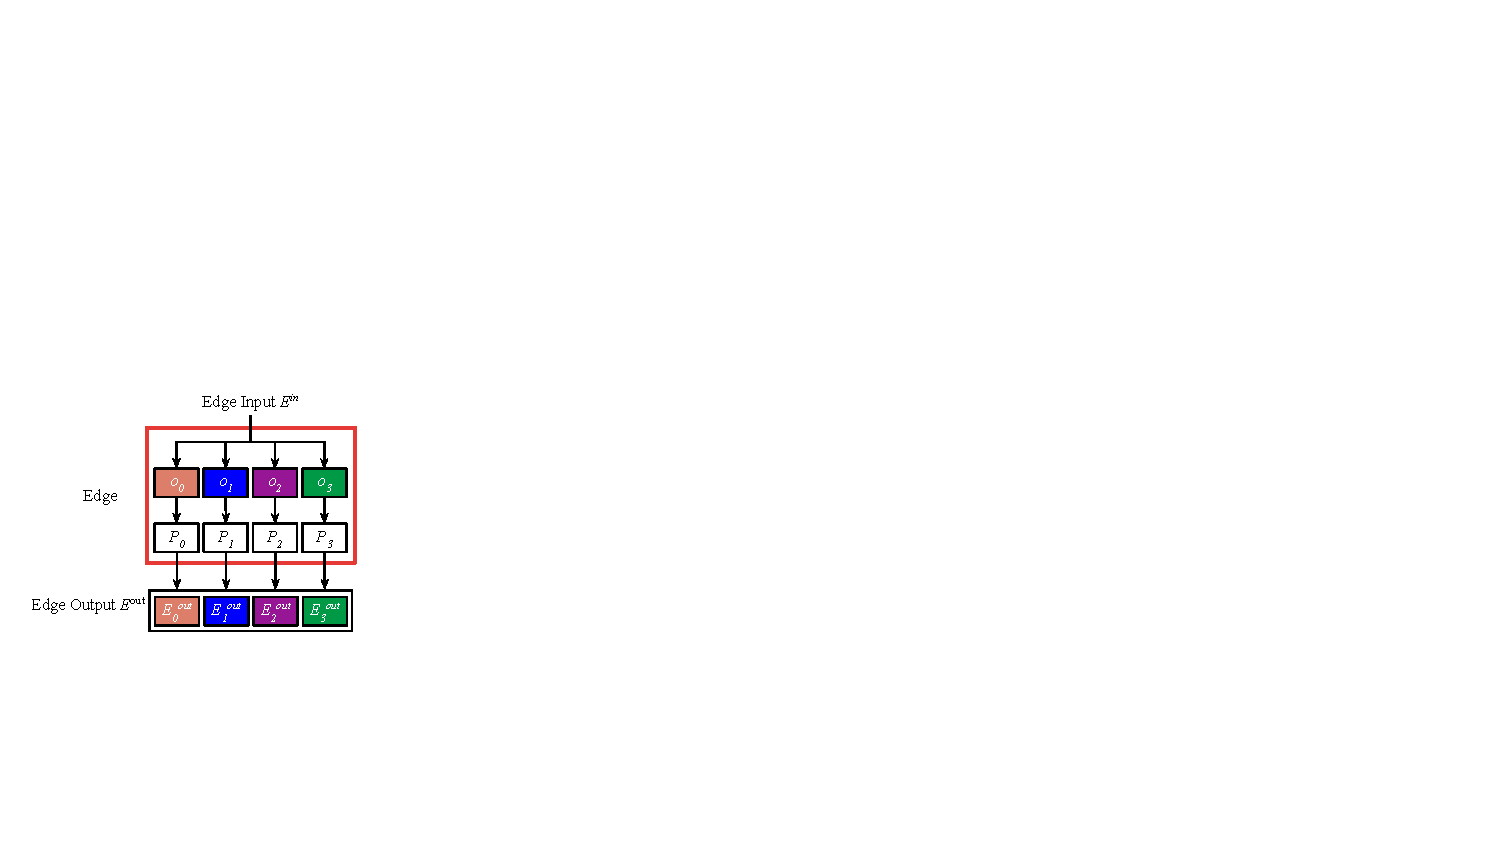
\includegraphics[width=.6\textwidth]{edge}
	\caption[Bonsai edge where $|\mathcal{O}|=4$]{Edges take some single input and pass it through $|\mathcal{O}|$ parallel operations.
The results of these operations are then individually pruned, and the edge outputs a list of these pruned operation outputs. These special
	edges that perform the parallel pruning are represented in red, while black edges simply transfer data unmodified between network nodes.}
	\label{fig:bonsai_edge_mainbody}
\end{figure}
\begin{figure}[ht!]
	\centering
	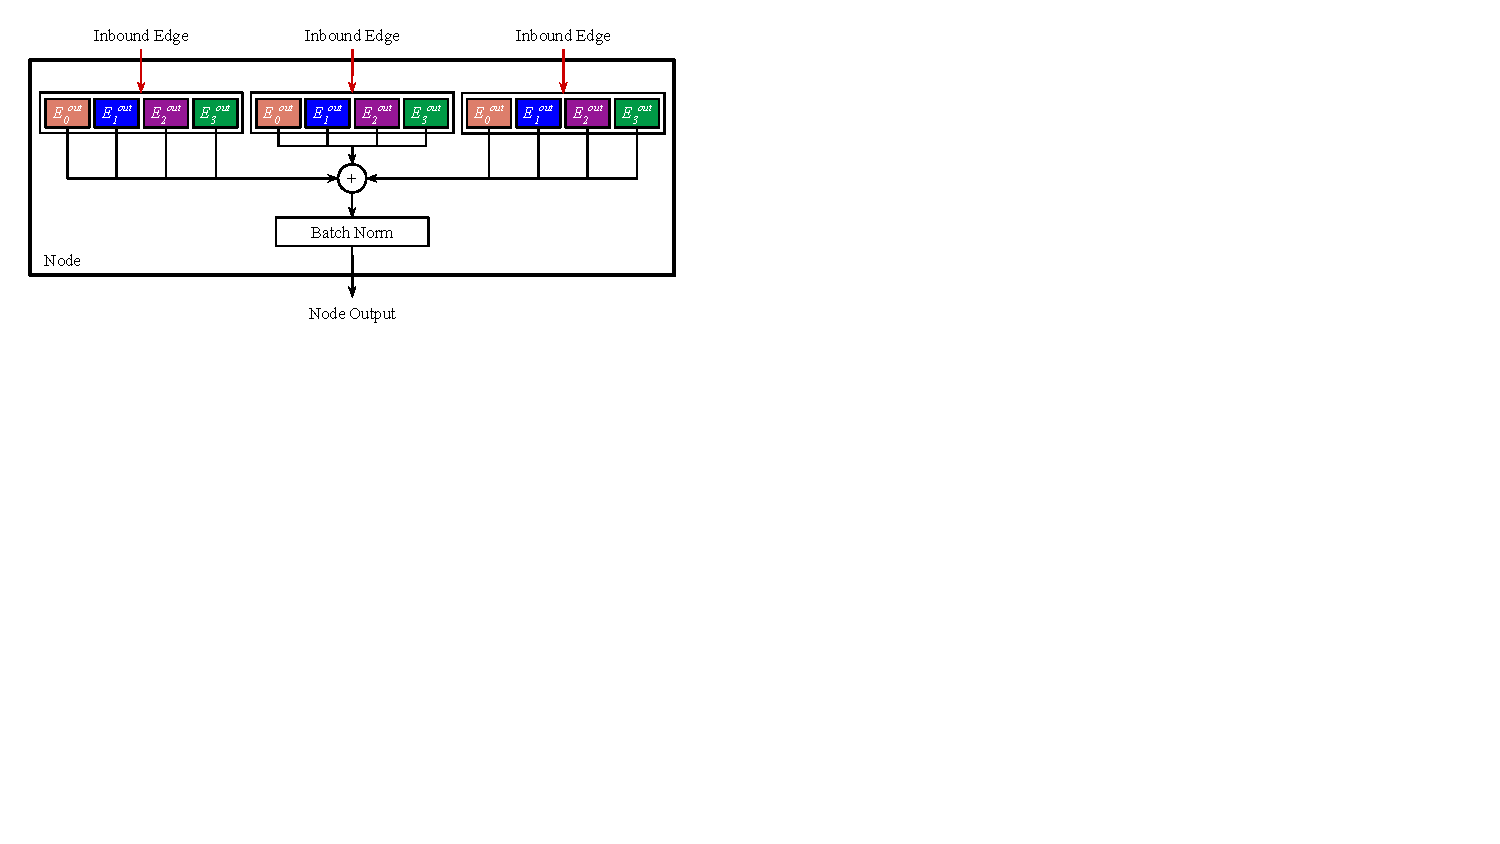
\includegraphics[width=\textwidth]{node}
	\caption[Bonsai node with three inbound Bonsai edges and $|\mathcal{O}|=4$]{
		Nodes concatenate the output lists of each inbound node via summation and batch normalization, and then pass this
concatenation on as the node output. This particular Bonsai node has three inbound Bonsai edges and $|\mathcal{O}|=4$.}
	\label{fig:bonsai_node_mainbody}
\end{figure}

Next, the total number of
cellular inputs is expanded such that each cell $C^c$ receives two inputs, the first from the previous cell and the
second from any combination of previous cells or the original model input $x$:
\begin{align}
	C^{in_1}_c &= C^{out}_{c-1} \\
	C^{in_2}_c &= \alpha_c^0 \, x + \sum_{i=1}^{c-1}{\alpha_c^i \, C^{out}_{i}} \label{eq:input_weights}
\end{align}

\noindent where $\alpha_c$ is a binary vector of size $n$. These transformations happen in the \textit{cell input handler}, which
is shown in Figure~\ref{fig:bonsai_ih_mainbody}.

\begin{figure}[ht]
	\centering
	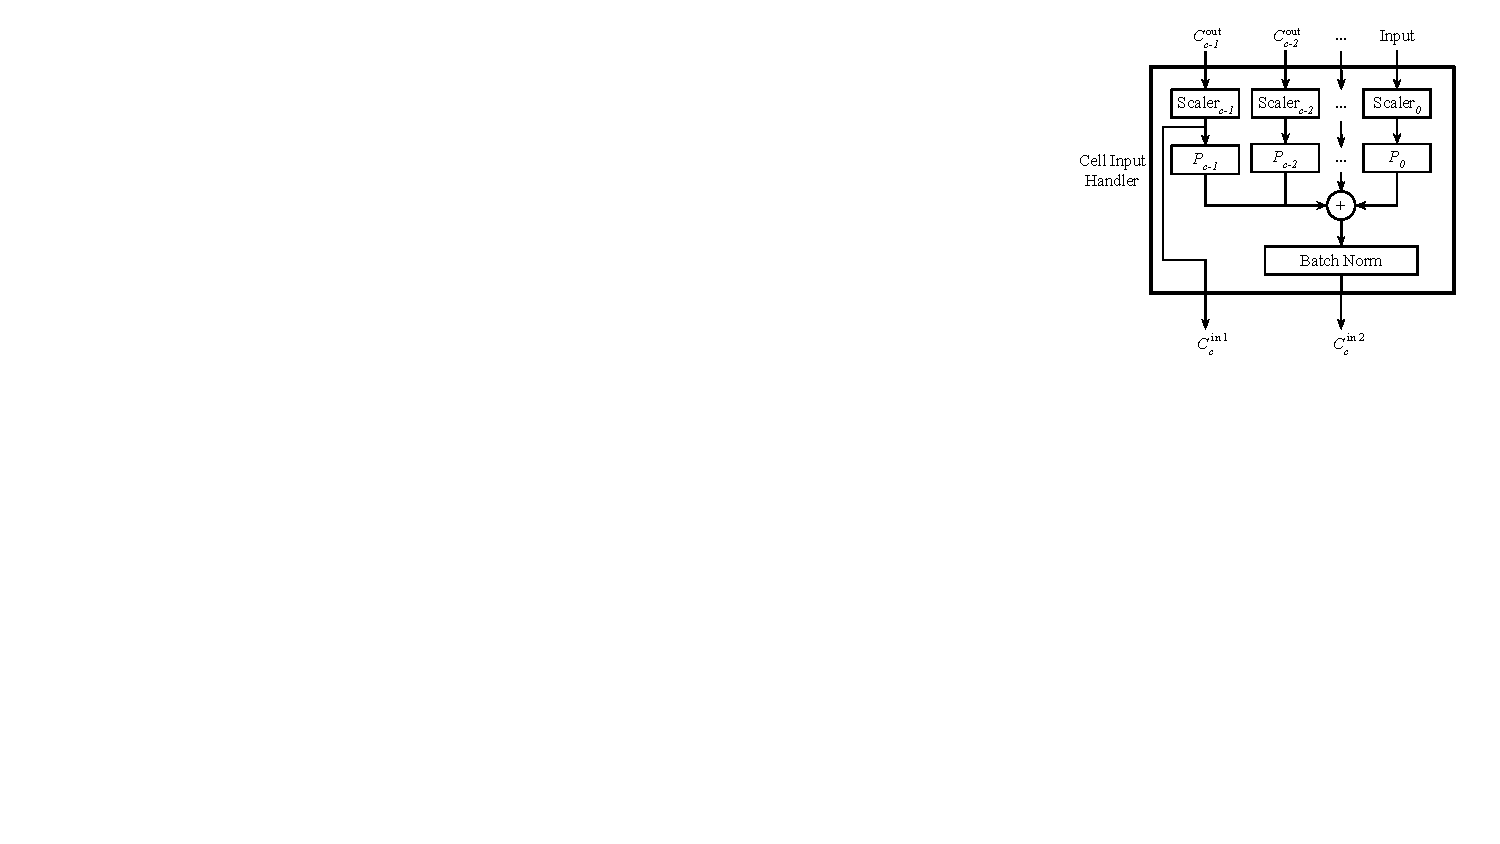
\includegraphics[width=.5\textwidth]{input_handler}
	\caption[The cell input handler]{The cell input handler.  Its job is to scale the outputs of antecedent cells
	to be compatible with the operations in the cell and produce two outputs.
The first output is just the scaled output of the directly previous cell $C_{c-1}$. The second output is the pruned
sum of all antecedent cells [$C_{c-1}$, \dots, $C_{0}]$ as well as the original model input.}
	\label{fig:bonsai_ih_mainbody}
\end{figure}

In this configuration, the $cth$ cell of a model has
$2^c$ possible connectivity patterns, meaning that the total number of cellular connectivities for a model with $C$ cells
is $\prod_{c=0}^{C}{2^c}$. Finally, cellular heterogeneity is allowed, which lets each cell have a distinct
connectivity and operation set. See Figure~\ref{fig:bonsai_cell_mainbody}.
for an architectural diagram of a Bonsai cell, and Appendix~\ref{chapter:bonsai_architectures} for a review of all
architectural diagrams shown thus far.

\begin{figure}[t!]
	\centering
	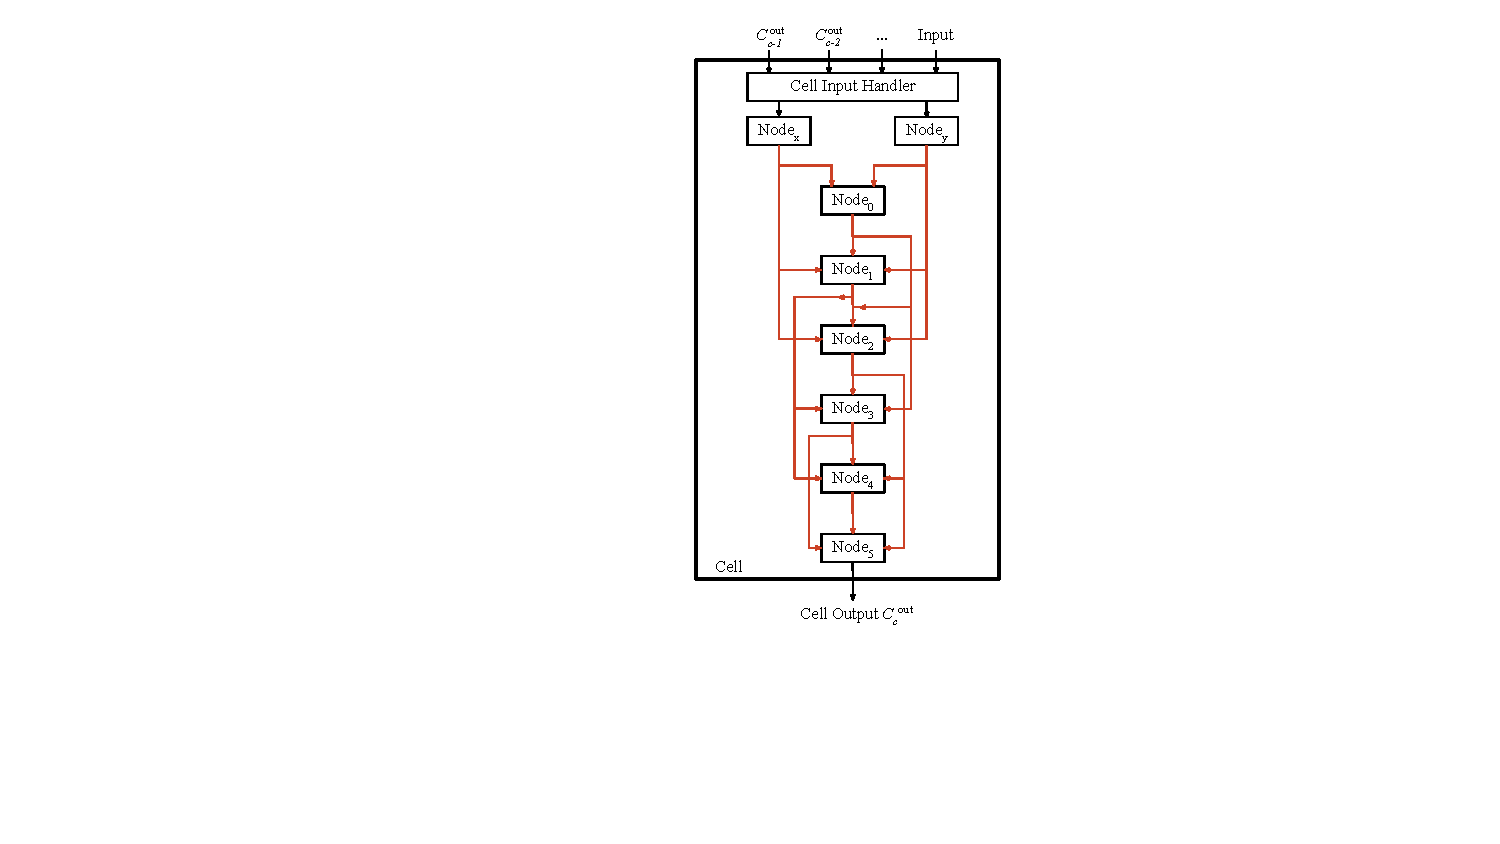
\includegraphics[width=.68\textwidth]{cell}
	\caption[Bonsai cell with six nodes and edge depth $d=3$]{Bonsai cell with six nodes and edge depth $d=3$. The two outputs of the
	cell input handler are passed to the input nodes of the cell, called Node x and Node y. From here, each node $n$ is connected via Bonsai
edges to each node $[n+1, n+2, \dots, n+d]$ where $d$ is the edge depth of the model. This simply controls the width/depth
ratio of the model; a depth of 1 means every node is linearly connected in serial, while a depth equal to the number of
nodes means each node connects to every downstream node.}
	\label{fig:bonsai_cell_mainbody}
\end{figure}


The difference in search space size between the constricted DARTS space and the Bonsai space is summarized in
Table~\ref{tab:space_size_general}.
\begin{table}[h]
\begin{center}
\begin{tabular}{c|ccc}
Space & \#Inter-cell Cnx & \#Intra-cell Cnx & \#Unique Cells \\
\hline
DARTS  & 1 & $|\mathcal{O}|^{\binom{N}{2} + 2N} $ & 2 \\[.5em]
Bonsai & $\prod_{c=0}^{C}{2^c}$ & $2^{|\mathcal{O}|^{\binom{N}{2} + 2N}}$ & C \\[.1em]
	\hline  \\[-1em]
DARTS (C=10, N=4, $|\mathcal{O}|$=7)& 1 & $6.8x10^{11}$ & 2 \\[.5em]
Bonsai (C=10, N=4, $|\mathcal{O}|$=7) & $3.6x10^{16}$ & $1.2x10^{21}$ & 10
\end{tabular}
\end{center}
\caption[Search space sizes of DARTS and Bonsai]{The total number of choices for each of the three design parameters in the DARTS and Bonsai search spaces, for
a generic model with $C$ cells, $N$ nodes per cell, and $|\mathcal{O}|$ operations, as well as the specific model configuration
used for CIFAR-10 in the DARTS paper.}
\label{tab:space_size_general}
\end{table}
In the specific DARTS CIFAR-10 search space described in the DARTS paper there are therefore roughly $4.6x10^{23}$
possible models, assuming a fixed pattern of normal and reduction cells.
The same configuration in the Bonsai space has $4.3x10^{222}$ possible models. With this dramatic increase in search space
size, evaluating neural search algorithms versus random search might be more elucidating, as the design restrictions
that may be artificially bolstering random search have been removed.

\section{Algorithm Design Considerations} \label{sect:alg design considerations}
Given the various advantages of one-shot, differentiable approaches as described in Section~\ref{sect:litreviewconclusion}, it was a natural choice to design one for this search space.
However, the predominant difficulty arising from these types of algorithms is that they tend to revolve around whittling down
a single architecture from some supernet that needs to fit entirely into GPU memory. The problem
with this is that a supernet is more expensive than a single path model by a factor proportional to the size of the
operation search space $\mathcal{O}$ because each edge is \textit{superconnected}; containing every operation within
$\mathcal{O}$ in parallel. Computing these parallel paths is costly in both floating point operations and memory
space, and drastically limits the size of supernets that are feasible on modern consumer hardware. Furthermore,
if a supernet was constructed that exactly fits onto a given GPU, any subgraph model extracted from that
supernet will be roughly $|\mathcal{O}|$ times smaller and therefore be utilizing only $\approx\frac{1}{|\mathcal{O}|}th$
of the computing power and memory available. This means that the subgraph model
will likely compare poorly against a model that takes more advantage of the GPU's power, as is suggested by the
`bigger-is-better' results from papers like ResNet~\citep{he2015}.

The cellular homogeneity present in many differentiable NAS algorithms like DARTS is arguably a compromise to
account for these exact problems; DARTS does not search for entire architectures via the supernet, but rather for single
cells. The single-cell supernet can be made as large as can fit on the GPU, and the space freed after subsequently whittling
the supernet down to some subgraph can then be used for subsequent stacking of the found cell. However, this comes at the
cost of only searching for a single cell, which then forces the algorithm to rely on the assumption that the best cell
will indeed stack into the best architecture, which is an assumption with no apparent justification in literature.
Much like~\cite{cai2018}, I find it dubious that
the best architecture for the first cell in the network would be the same as that for the 10th, and so examining this
claim is a secondary motivation for this work.

To design a one-shot differentiable algorithm that allows for cellular heterogeneity, as well as the other
two properties of the Bonsai space, two components are necessary. First is a method of \textit{pruning},
some differentiable method to trim the supernet down into optimal subgraphs. Next is a \textit{cell search} algorithm,
some way to uniquely search for each cell in the network, in such a way that each cell was aware of
its position in the network and its antecedents.

\section{Pruning}\label{sect:pruner_introduction}
While the DARTS approach of performing a weighted sum of each candidate operation
and using the softmax of the weights to determine the final operation selection is a valid pruning approach, it is one
implicitly designed around single-path edges. In theory, you could keep the weighted sum of operations and remove the softmax,
instead ranking operations by their weight and preserving the $n$ most highly weighted. This however creates a variety of
new issues, namely how should each edge pick $n$? Instead, some way of differentiably and dynamically selecting
operations was necessary, such that each edge could choose which and how many operations it needed given its particular needs. Such a component
materialized in the Differentiable Pruner, introduced by \citeauthor{kim2019v2} in the 2019 paper
\hyperlink{cite.kim2019v2}{``Differentiable Pruning Method for Neural Networks''}\footnote{Now titled ``Plug-in,
	Trainable Gate for Streamlining Arbitrary Neural Networks''}.

The differentiable pruner was originally introduced as a means of pruning floating point operations (FLOPs) from neural operations, specifically to
reduce the size of fully-connected layers inside of neural networks. The authors describe the problem of attempting to
prune these connections via a simple gate function (like the Heaviside step function, for example) as similar to the
vanishing gradient problem seen in sigmoid activations in regions far from 0. This problem is illustrated by applying
the simple gate to a 1-D example, where the gate $G$ has a single weight $w$ that controls whether the input tensor passes
through the gate or not:
\begin{align}
	G(x, w) &= \begin{cases}
				0 & w<0 \\
				x & w\ge 0
	\end{cases}
\end{align}

When $w$ is less than zero the gate is closed, whereas the gate is open when $w$ is greater than or equal to zero.
However, the gradient of this gate function with respect to the weight is zero everywhere, meaning there is no
information for gradient descent to use in the process of learning $w$. This means that regardless of the downstream
effects of the tensor passing through the gates the gate will always remain in the exact position it is initialized in.
To remedy this, the authors add a saw wave $S$ of some small amplitude $\frac{1}{M}$ to the gate function $G$,
creating the differentiable pruner function $P$:
\begin{align}
	G(w) &= \begin{cases}
						0 & w<0, \\
						1 & w\ge 0
					\end{cases} \label{eq:gate} \\
	S(w) &= \frac{M w - \lfloor M w \rfloor}{M} \label{eq:saw}\\
	P(x, w) &= (G(w) + S(w)) x
\end{align}

\begin{figure}[ht!]
	\centering
	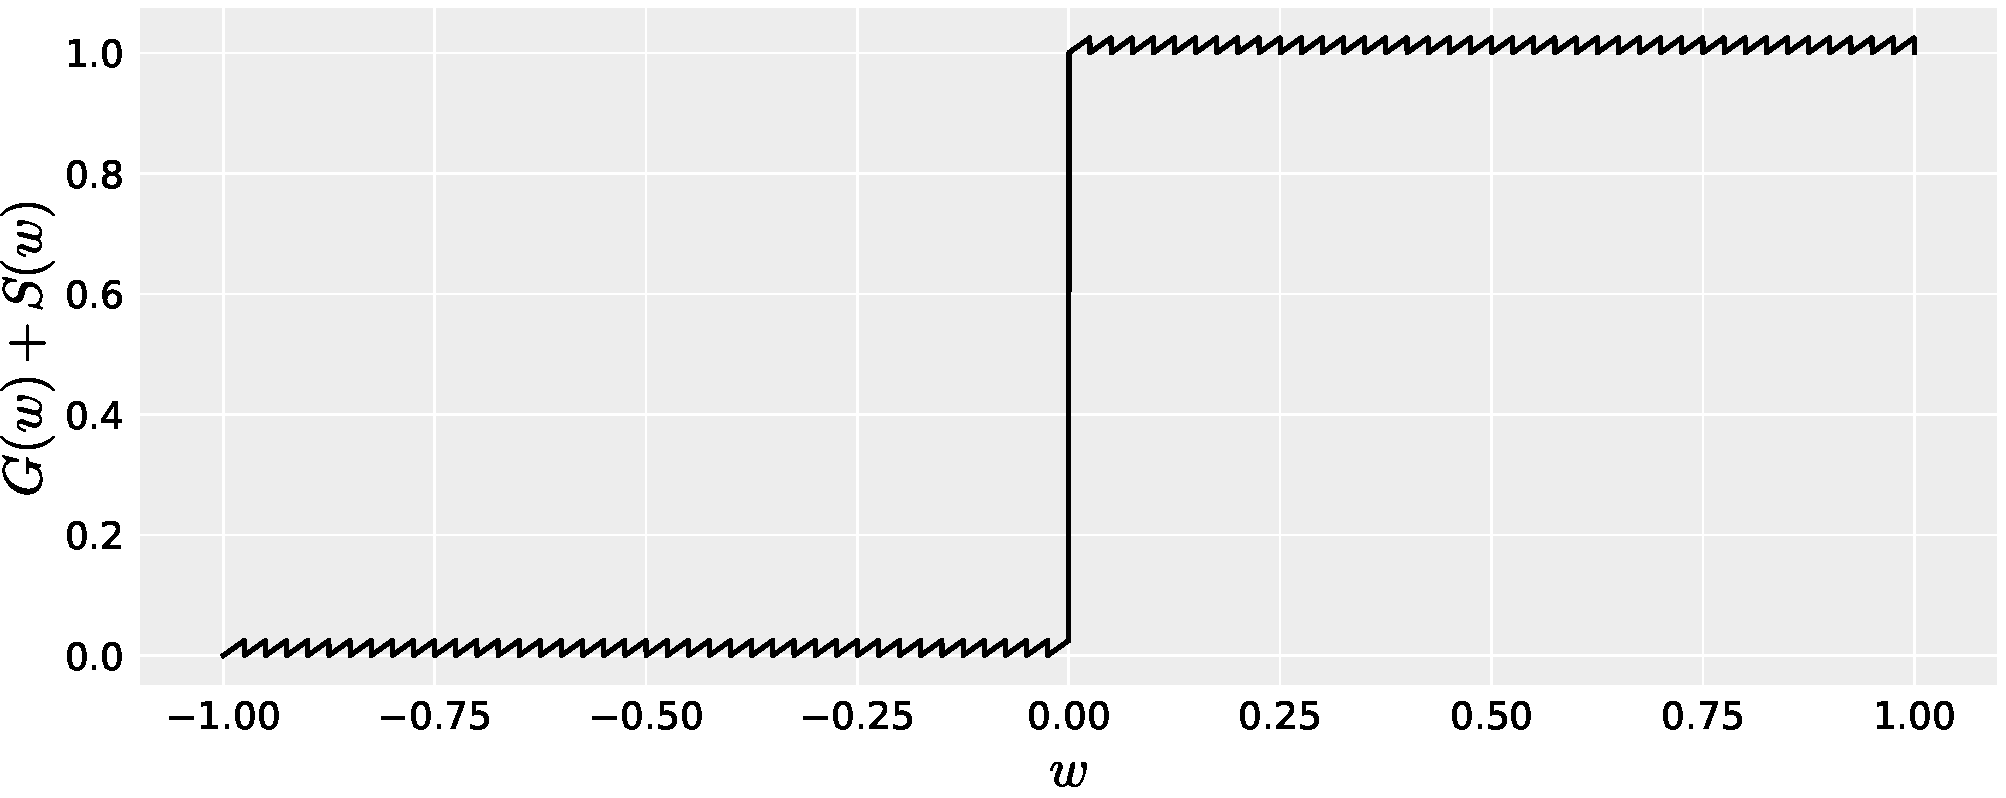
\includegraphics[height=12em]{pruner}
	\caption[The differentiable pruner function, plotted]{The pruner equation $G(w)+S(w)$, with M chosen to be large enough to be perceptible.}
	\label{fig:pruner}
\end{figure}


With large enough $M$, $S(w)$ is effectively 0 everywhere while still having
a constant gradient of 1 with respect to $w$. Adding this saw to the gate creates a function with the
multiplicative properties of the gate that maintains the gradient properties of the saw wave, as visualized in
Figure~\ref{fig:pruner}.


The reasoning behind the design of the differentiable pruner can be justified by comparing its gradient descent behavior
against that of a simple gat in a short experiment. To start the experiment, the weights of both the simple gate and the differentiable pruner are initialized at
0.1, meaning both functions start in the open position. Then the weights are updated via gradient descent given the following
loss function $\mathcal{L}$:
\begin{align}
	\mathcal{L} = (P(x, w) - y_{target})^2
\end{align}

Within this specific example, $y_{target}$ is set to 0 for the first 50 gradient steps, meaning that the loss minima will occur when each function is in the
closed position and thus outputs $0$. For the next 50 gradient steps $y_{target}$ is set to $x$, which instead means the loss
minima will occur when the functions are in the open position and output $x$. The progression of each function's weight
can be seen in Figure~\ref{fig:gatevspruner}.


\begin{figure}[ht]
	\centering
	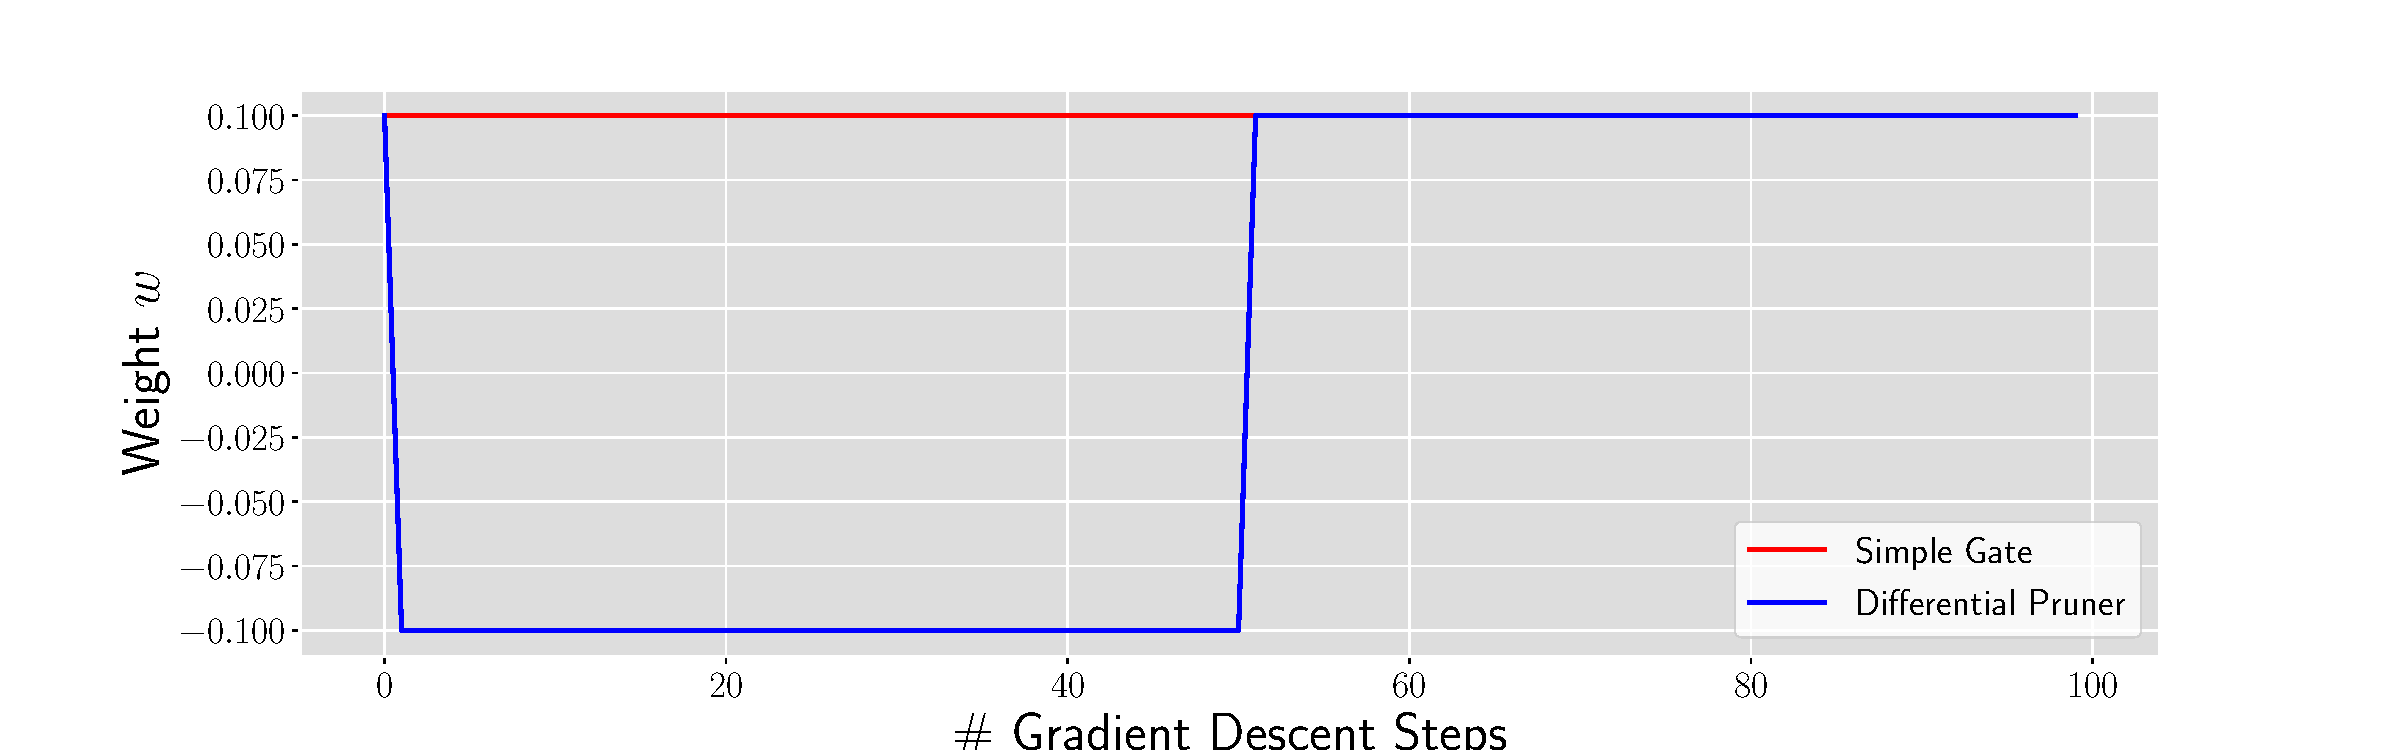
\includegraphics[width=\textwidth]{gate_vs_gateandsaw}
	\caption[Gradient descents of simple gates versus differentiable pruners]{Gradient descent of a simple gate (red) compared to the differentiable pruner (blue).
	The first 50 steps
	of gradient descent incentivize a closed gate. The second 50 steps instead reward an open gate.}
	\label{fig:gatevspruner}
\end{figure}

Notice that the differentiable pruner quickly learns the desired gating, while the simple gate does not learn at all. This
demonstrates both claims; first that a simple gate cannot train by backpropagation and second that the differentiable
pruner manages to remedy this problem.

To use the differentiable pruner to perform supernet pruning, differentiable pruners are placed along every
candidate edge in the supernet, meaning that every value within
$\alpha_o$ and $\alpha_c$ from equations~\ref{eq:op_weights} and~\ref{eq:input_weights} is computed by a separate
pruner. The operation that is performed along the operation edges is as follows:
\begin{align}
	E^{out} = \sum_{o \in \mathcal{O}} P_o (o(E^{in}), w_o)
\end{align}
Along cellular input edges, the calculation is:
\begin{align}
	C^{in_1}_c &= C^{out}_{c-1} \\
	C^{in_2}_c &= P^c_0(x, w^c_0) + \sum_{i=1}^{c-1}{P^c_i(C^{out}_{i}, w^c_i)}
\end{align}

\subsection{Deadheading}
As the supernet trains, each of the pruners can operate independently to preserve or prune the edge that they
lie along. However, the pruners simply perform a virtual gating of their respective operations; a closed pruner is simply a multiplication by zero, but the operation along the
edge is still calculated and takes up space in memory. To actually free up computational resources, the decision of the
pruner must be cemented by transforming the purely mathematical deletion into a physical one through \textit{deadheading}.
Deadheading entails removing the entire edge that the pruner operates on, such that the
candidate operation is permanently removed from the supernet. Henceforth a pruner moving to an `off' position
will be referred to as a \textit{soft} pruning, whereas deadheading and deletion is a \textit{hard} pruning.

\begin{figure}[ht!]
	\centering
	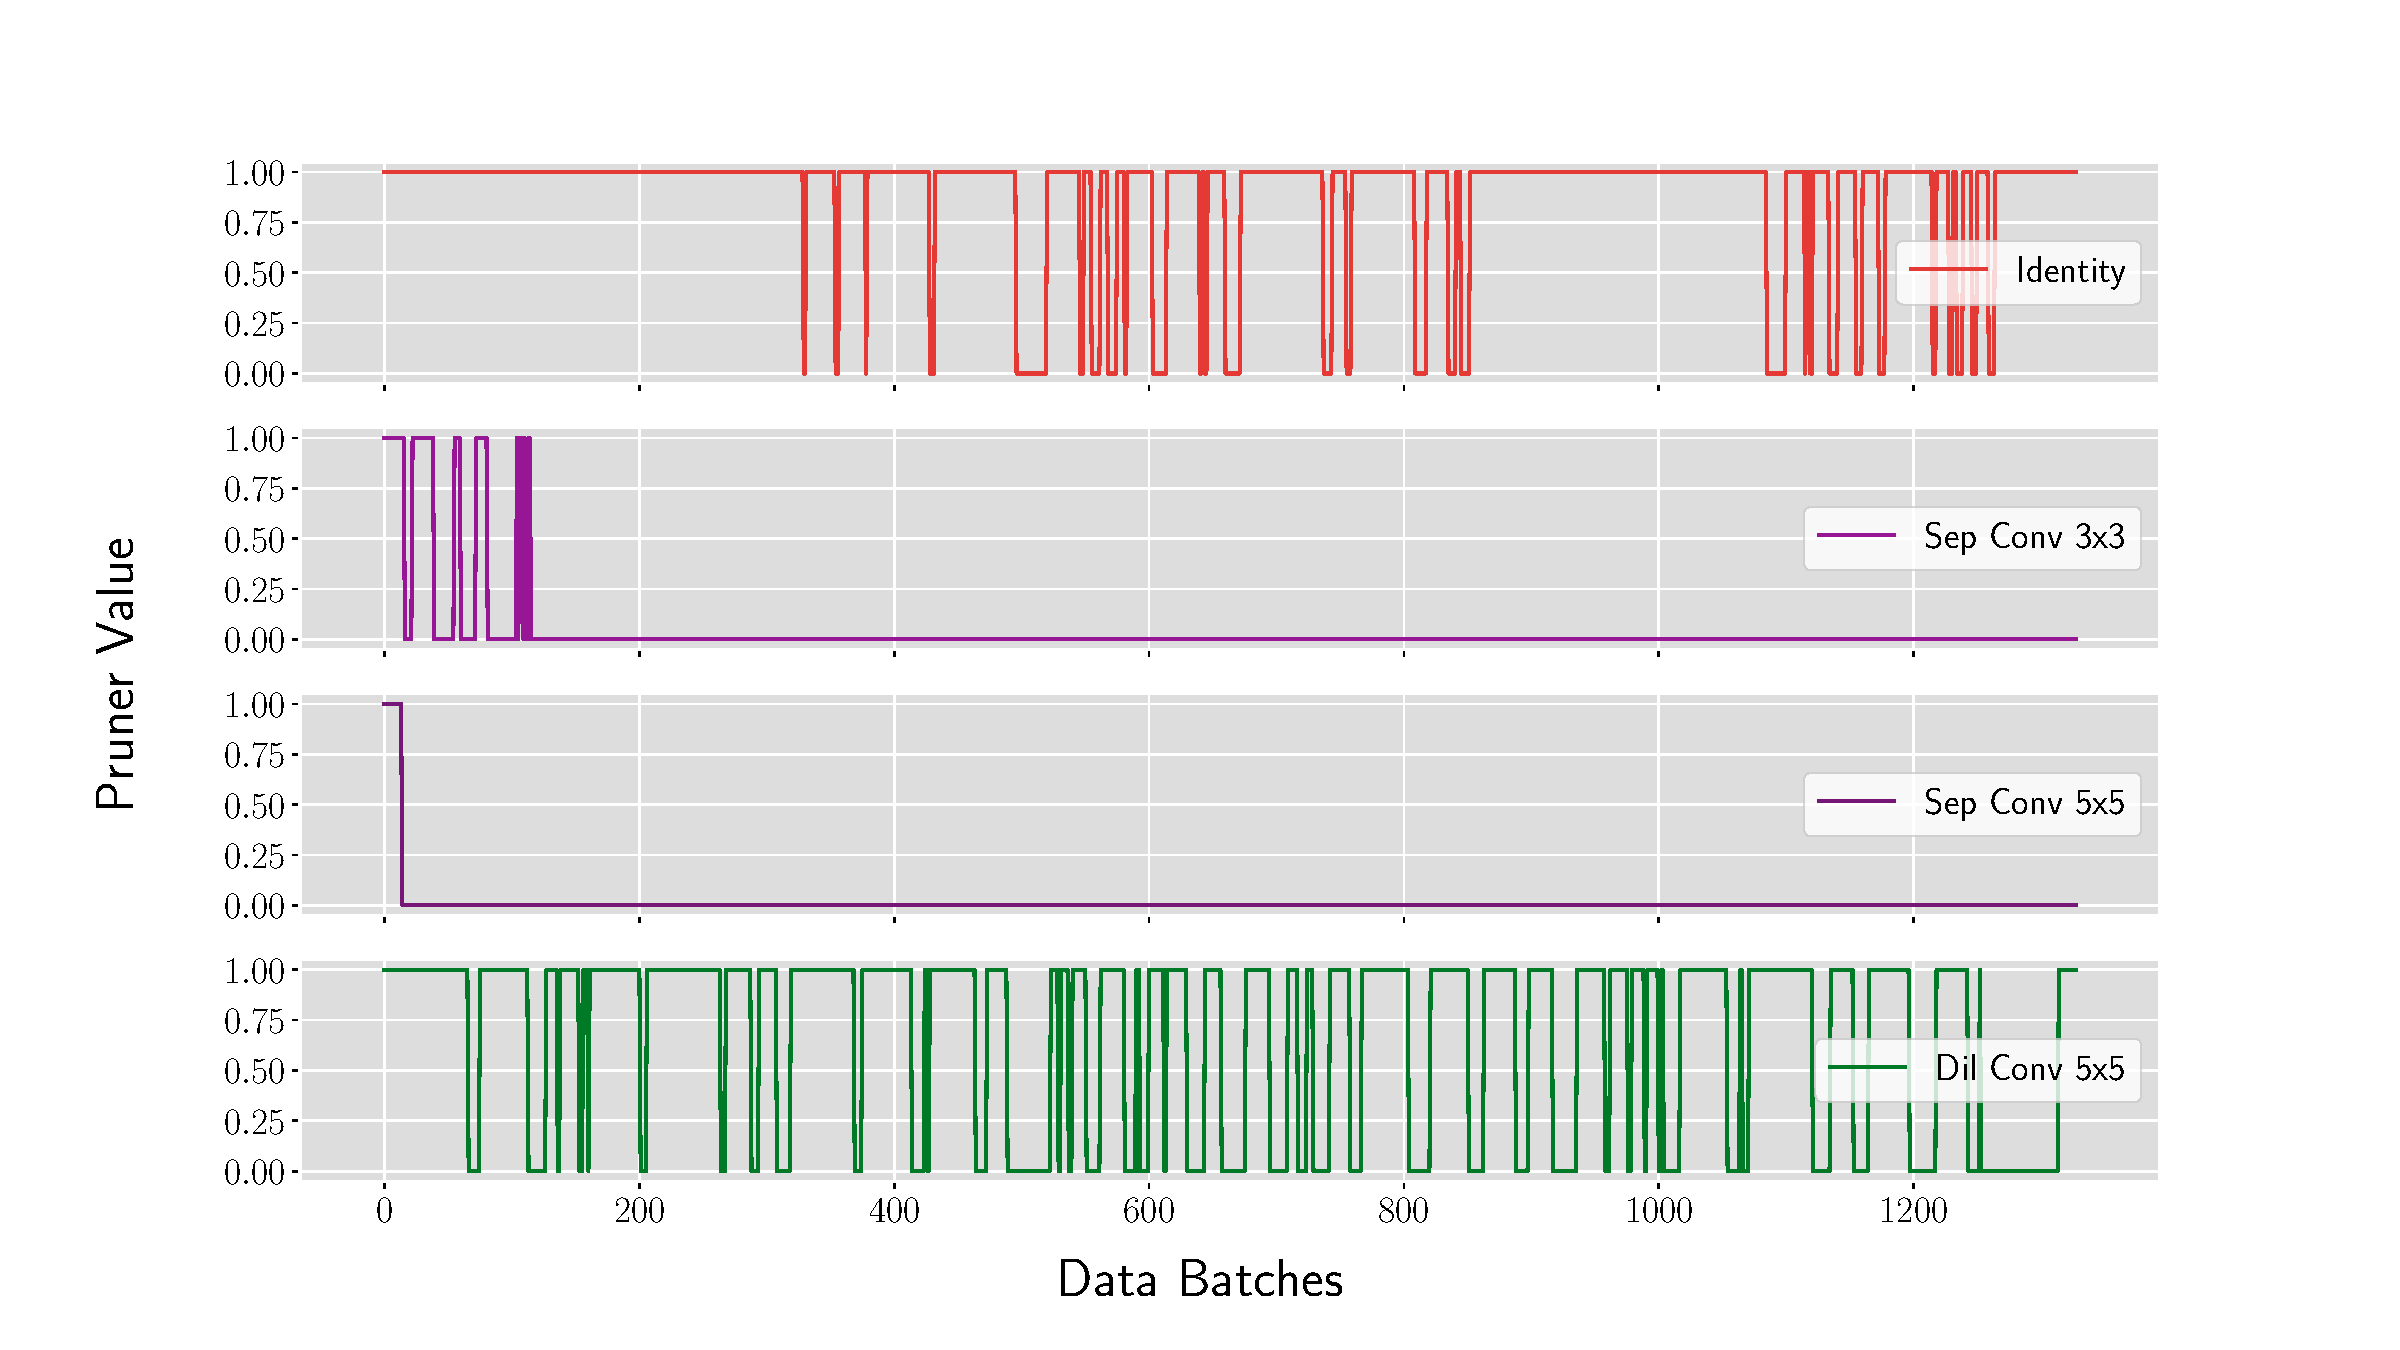
\includegraphics[width=\textwidth]{pruner_history}
	\caption[Pruner values of different operations over time in a CIFAR-10 BonsaiNet model]{Pruner values over the first 1,300 data batches of four edges within a CIFAR-10 Bonsai model. Notice
	 the toe-dip behavior of the identity and 5x5 dilated convolution edges, where they toggle repeatedly between on
	and off states as the model experiments with their inclusion. The separable convolution edges however exhibit the
	permanent-off behavior, where after staying switched off for multiple data epochs they never switch back on.}
	\label{fig:prunerhist}
\end{figure}

To perform deadheading effectively, a policy must be designed that rapidly and accurately identifies edges that the model
no longer needs. The faster this decision can be reached, the faster
the search process can occur. The more accurately this decision can be made, the better the performance of the search
algorithm. Designing a deadheading policy is thus balancing these two aims; too eager and risk removing valuable model
edges, too conservative and the supernet will never prune.

Crucial to the design of every iteration of deadheading policy was the observation that pruners tend to exhibit
one of three common behaviors: permanent-on, toe-dipping, or permanent-off.  These latter two behaviors can be
observed in Figure \ref{fig:prunerhist}.  My hypothesis as to why these three behaviors are so common revolves around
a phenomenon I call \textit{operational codependency}. As a model trains, an operation's weights will be learned such
as to complement the other operations that it interacts with. As such, each operation will tailor its output such that
in collaboration with other nearby operations it performs effective tensor transformations. If the
configuration of these operations changes, by something like a pruner switching off one of these neighboring operations
or reintroducing one that had been switched off, this codependance breaks. The operation weights are tailored to a particular
operational coalition that no longer exists, which is likely to be significantly detrimental to the model's performance if the
operation's output is nonzero. Once a
model has training in a specific configuration for long enough, operation codependance arises and `burns-in' the model
configuration, which means it is unlikely to find success altering the configuration. This is what causes the permanent-on
and permanent-off behaviors of pruners; their local neighborhood of operations has burnt in and thus any change to the
pruner state is exclusively detrimental.

On the other hand, when an operation's local neighborhood is in constant flux, with operations switching on and off
rapidly, the operations do not form codependence as they simply cannot rely on the nearby operations being consistent.
As such, pruners in such a neighborhood can freely `dip their toes' into either state with little penalty,
frequently experimenting and toggling between on and off.
The deadheading policy needs to identify permanent-off edges to remove from the model, while preserving permanent-on
edges and allowing toe-dipping edges to experiment.

The first few iterations of the deadheading policy were based solely around identifying permanent-off operations, with
the first iteration tracking each pruner's state at the end of each training epoch. Every $n$ epochs, the deadheading operation triggers,
and deadheads all edges where their pruner was off at the end of the majority of the last $n$ epochs and off at the end
the most recent one. There is an implicit inefficiency in this design, which concerns the fixed window of state sampling.
Since the state of the pruners is sampled in a $n$ epoch window every $n$ epochs,
it is possible to run into cases where a pruner's decision to move to a permanent off state straddles two windows. This would mean
waiting for an entire additional $n$ epoch cycle to deadhead the edge. This is remedied by adopting a sliding window
policy, wherein the deadhead policy is triggered each epoch and look at the previous $n$ epochs. Within this sliding window,
the same deadhead criteria as before is maintained: off in the last epoch and in the majority of the epochs. The sliding window
policy was the second iteration of the deadheading policy that was tried for BonsaiNet, and the difference between the
two policies' efficacy can be seen in Figure~\ref{fig:dhwindow}.

\begin{figure}[ht!]
\centering
\begin{subfigure}{.5\textwidth}
  \centering
  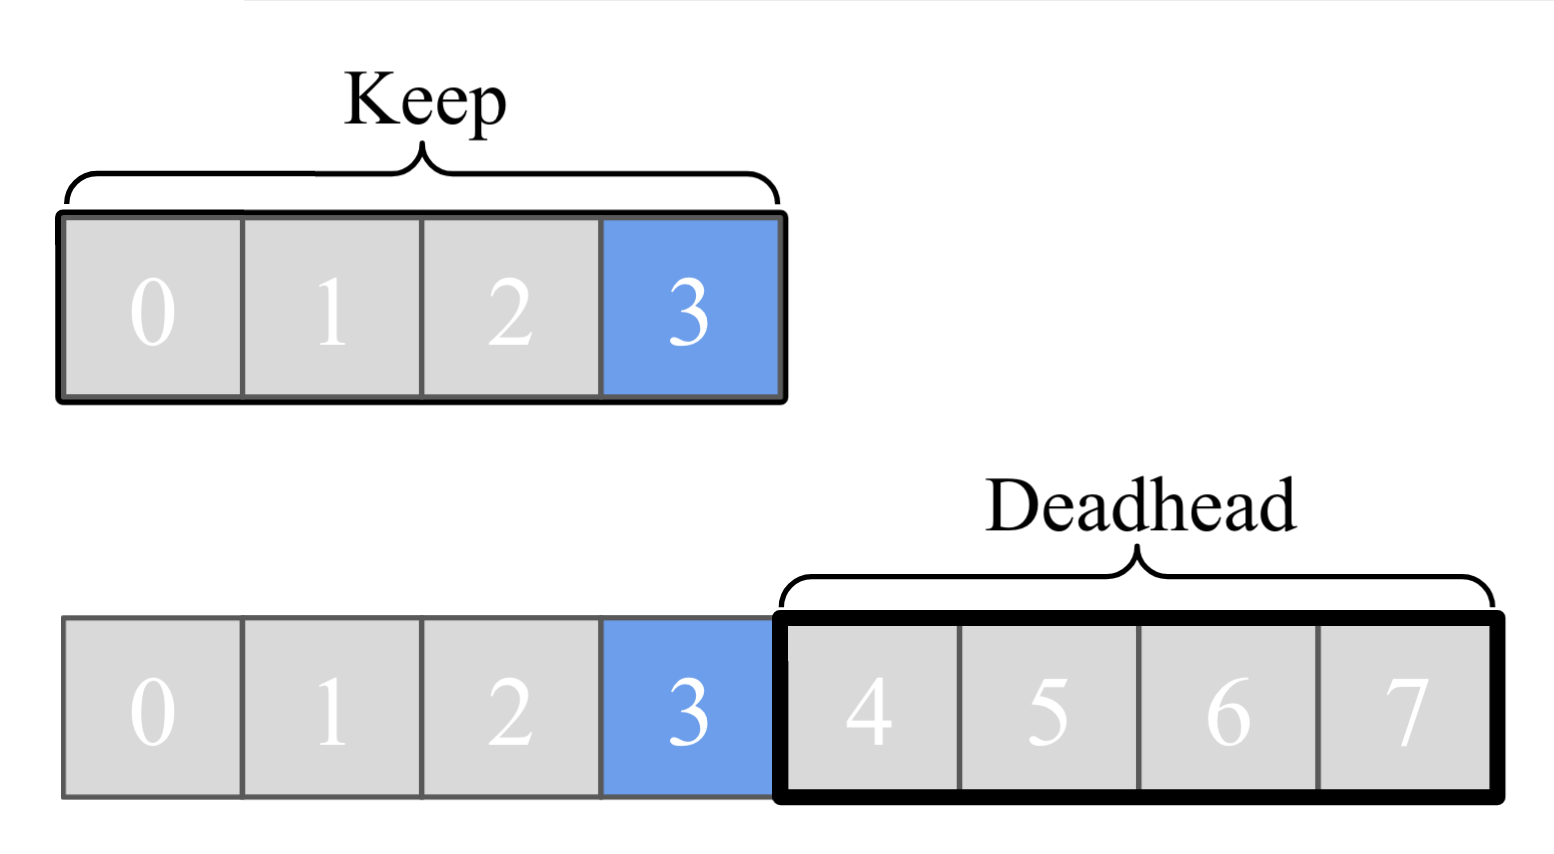
\includegraphics[width=\linewidth]{dh/fixed}
  \caption{Fixed window policy}
\end{subfigure}%
\begin{subfigure}{.5\textwidth}
  \centering
  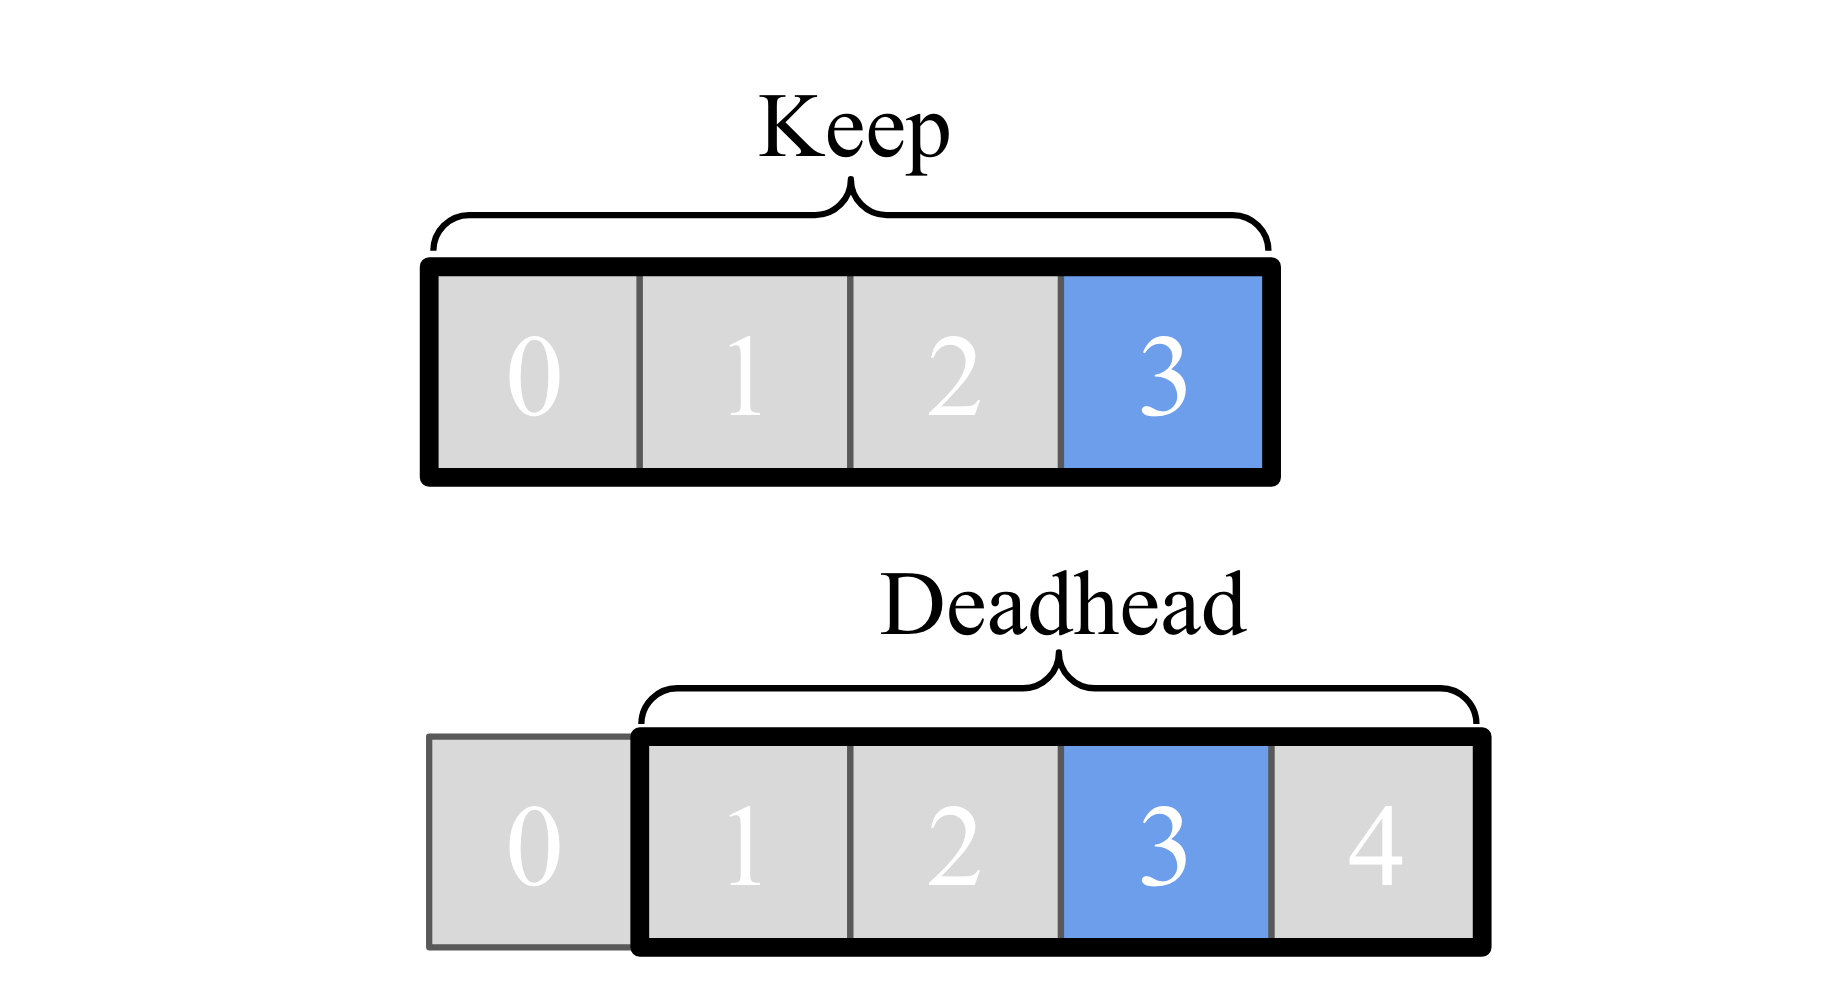
\includegraphics[width=\linewidth]{dh/sliding}
  \caption{Sliding window policy}
\end{subfigure}
\caption[Comparison of fixed and sliding window deadhead policies]{Comparison of a fixed and sliding window deadhead policy with a window size of 4 epochs. The edge being evaluated
	is on at the end of epoch 3 as shown by the blue block, but off after every other epoch.
	In this case, the fixed window policy needs 8 epochs to reach a deadheading decision, while the sliding window
	only needs 5.}
\label{fig:dhwindow}
\end{figure}

While the second iteration is definitely more time-efficient than the first, both share a fundamental flaw in practice.
Since gradient updates happen on a per-batch basis, not per-epoch, there are multiple
hundred gradient updates per epoch, and thus multiple hundred pruner states per epoch. Sampling just the final epoch state
means the deadheading decision is based on a tiny fraction of the pruner state, which is unlikely to be meaningfully
representative of the overall state. This could result in the epoch-end sampling producing a very
misleading picture of the pruner's state history, and could potentially cause a deadheading policy to make decisions that
do not align with how a model values an edge. For example, imagine a toe-dipping pruner that is more or less randomly fluctuating between
states, but happens coincidentally to be always off at the end of epochs. Such an edge would be pruned from the model,
despite the pruner making no such concrete decision. The worst case are scenarios where a per-epoch sampling policy
would produce diametrically opposed decisions to that of how a model truly values an edge, and these scenarios are explored in
Figure~\ref{fig:dhbatch}.

\begin{figure}[ht!]
\centering
\begin{subfigure}{.5\textwidth}
  \centering
  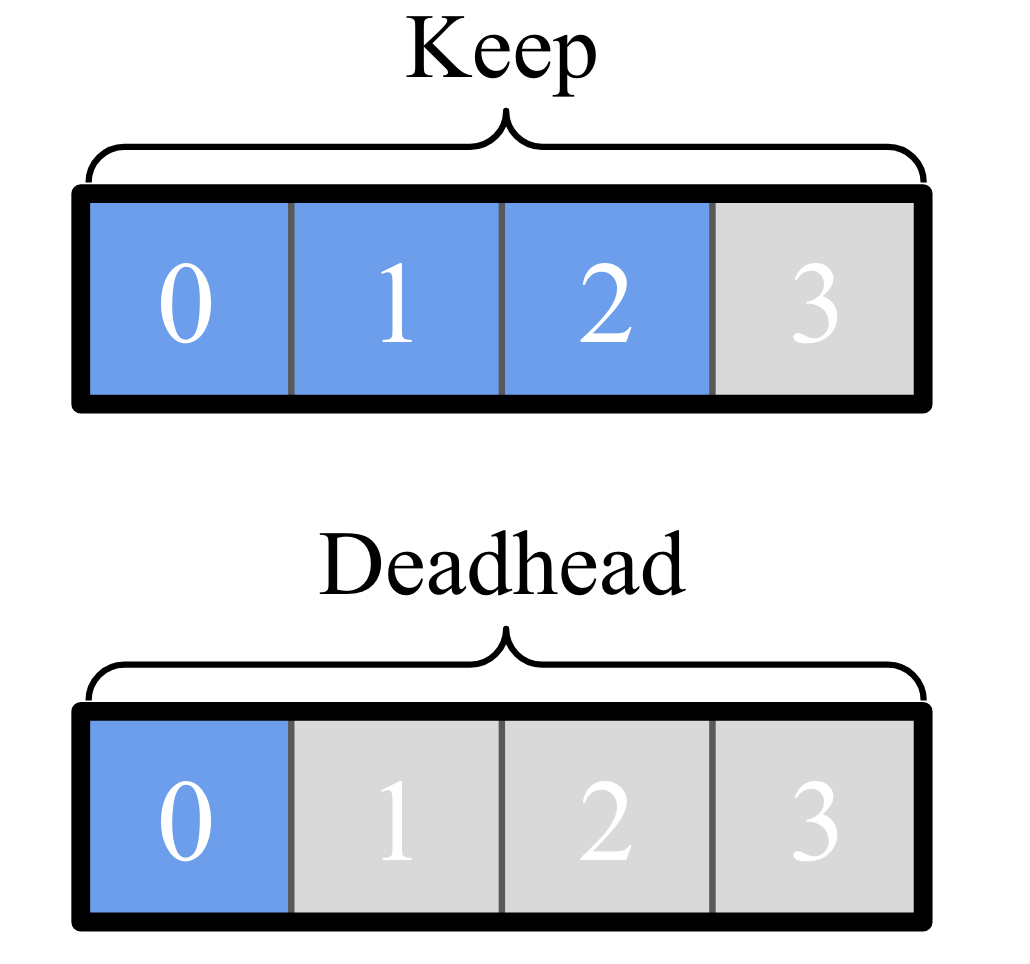
\includegraphics[width=.6\linewidth]{dh/epoch}
  \caption{Epoch-end sampling policy}
\end{subfigure}%
\begin{subfigure}{.5\textwidth}
  \centering
  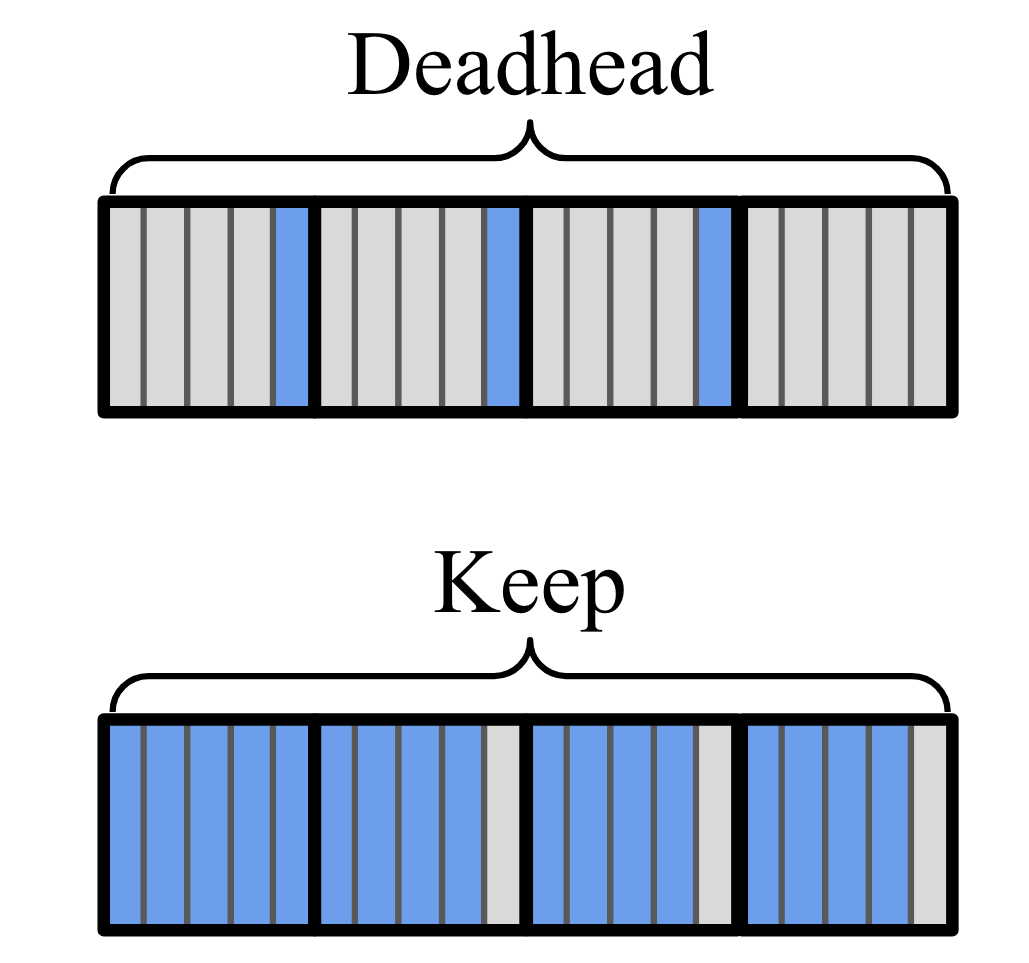
\includegraphics[width=.6\linewidth]{dh/batch}
  \caption{Per-batch sampling policy}
\end{subfigure}
\caption[Comparison of worst-cast scenarios of epoch-end sampling policy]{Comparison of worst case scenarios for the epoch-end sampling policy. In the first case, the pruner is off 85\%
of the time, only on at the end of epochs 0, 1, and 2. A per-epoch sampling policy would preserve this edge, while a
per-batch policy would deadhead it. In the second case, the exact opposite occurs.}
\label{fig:dhbatch}
\end{figure}

 The final iteration of the deadheading policy uses both a sliding window and per-batch sampling, combining the speed
advantages of the sliding window with the accuracy benefits of per-batch sampling. In this final iteration, the pruner
states from each of the $b$ batches within the previous $n$ epochs are sampled, for a total of $bn$ pruner states. If a
pruner is on for less than 25\% of those pruner states, the pruner is deadheaded. This 25\% figure was chosen arbitrarily,
and while it works well in practice it could be interesting to explore the efficacy of other possible options.

An example of this behavior exists in the pruners from Figure~\ref{fig:prunerhist}, which shows a snapshot of 1300 states for the four pruners. If the deadhead window
spans the entire 1300 states, the final deadheading policy would keep the identity and dilated convolution, with those
pruners remaining on for 87.3\% and 66.8\% of sampled states respectively. Both the 3x3 and 5x5 separable convolution would be
deadheaded, having been on for only 4.1\% and 1.1\% of sampled states.

\subsection{Compression}
While the mere presence of pruners in a model will allow the model to remove obviously bad edges, it will need
encouragement to perform more extensive pruning. This is due to codependence; models that keep a certain configuration
of operations for too long will be very reticent to remove any of them. By adding a mathematical reward in the loss function
for removing operations, the model is encouraged to experiment with removing operations. The process of experimentation
will prevent operations from becoming codependent, thus allowing them to be pruned even faster as the penalty for removal
is not particularly high. This reward is implemented by adding a \textit{compression} term to the loss
function, computed as follows:
\begin{align}
	\mathcal{L}_{comp} &= \lVert c - c_{tgt} \rVert \label{eq:comp_term}
\end{align}

\noindent Here, $\lVert . \rVert$ is the Euclidean norm, while $c_{tgt}$ and $c$ refer to the target and measured model
compression respectively, where compression is some measure of how many edges have been removed from the model compared
to its original state. There are a number of ways to measure this compression, and the
first version of \citeauthor{kim2019v1}'s differentiable pruner paper as submitted to ICML 2019
used differentiable parameters as the metric of choice. The original number of parameters in a model was compared to the number of parameters after pruning, and the ratio between the two is
the compression. For example, a model with 5 million parameters originally and 2 million parameters after pruning would have
a compression of $0.4$.

The issue with this metric revolves around the desired use for pruners. The intent is to trim down a supernet such
that VRAM space is cleared to later scale up the model, which means that reducing the VRAM usage of the existing supernet
is the primary goal. In this regard, not all parameters are created equal.

\begin{table}[h]
\begin{center}
\begin{tabular}{c|c|c}
Operation & \# Parameters & VRAM Size\\
\hline
Identity					& 0 & 14 MB\\
Max Pool 3x3				& 0 & 56 MB\\
Separable Convolution 3x3   & 3,384 & 112 MB\\
Separable Convolution 5x5   & 4,536 & 112 MB\\
\end{tabular}
\end{center}
\caption[Comparison of parameter count and VRAM size in megabytes of various tensor operations over identical input]{Comparison of parameter count and VRAM size of a variety of tensor operations over identical input.}
\label{tab:opcosts}
\end{table}
As seen in Table~\ref{tab:opcosts}, there is little correlation between parameter count and VRAM cost. While identities
and max pooling operations share the same parameter count of 0, they differ in VRAM cost by a factor of 4. Meanwhile, the
parameter counts of the separable convolutions differ by around 1,000, but they both take up 112B on the GPU. With a
parameter based compression metric, identities and pooling operations are `free' and are infinitely cheaper than any
of the convolutions. These operations would be unlikely to be pruned if such a metric was used in the compression term,
despite them still taking up space on the GPU.

A later update to \citeauthor{kim2019v2}'s differentiable pruner paper, published as a poster in AAAI 2020,
acknowledges this issue and changes the compression metric, instead comparing the FLOP ratio between the original model and the model post-pruning.
However, this is still not necessarily
correlated well to VRAM size, as a possibility can be imagined where an operation performs intense calculations
without needing to allocate new tensors in memory. The obvious solution to these correlation issues is to directly use
VRAM size as the compression metric. To do this, the VRAM cost of every edge in the model needs to be measured, which can
be greatly simplified by the fact that space allocation differences between operation in the model boils down to
three factors: the mathematical function the operation performs, the input dimensionality of the tensor passed to the
operation, and the stride of the operation. Operations that are identical across all three of those factors will have
identical VRAM size requirements, and thus all that is needed is to sample each operation in the model over every stride and
input dimensionality that could appear in the model. Normal cells will contain all $|\mathcal{O}|$ operations, each with
stride 1 and operating over a single input tensor dimensionality. Reduction cells will contain the same
$|\mathcal{O}|$ operations, the majority with a stride of 1 and operating over some input dimensionality $[C,H,W]$. The remaining
operations of a reduction cell handle spatial downscaling, and as such have a stride of 2 over an input dimensionality
of $[C,2H,2W]$. As such, a normal cell has a single edge input dimensionality, while reduction cells have two. Therefore,
for a model with $N$ cells, $R$ of which are reduction cells, there are a total of $|\mathcal{O}|((N-R)+2R)$
or $|\mathcal{O}|(R+N)$ operation sizes to sample. Figure~\ref{tab:allopcosts} shows the various measurements necessary
for a 3 cell, 2 reduction BonsaiNet model for CIFAR-10.

\begin{table}[h]
\begin{center}
\begin{tabular}{r|c|c|c|c|c}
	& \multicolumn{3}{c|}{Stride 1} & \multicolumn{2}{c}{Stride 2} \\
 & 36x32x32 & 72x16x16 & 144x8x8 & 72x32x32 & 144x16x16 \\
	\hline
Identity & 3.60 & 1.80 & 0.90 & 1.80 & 0.90 \\
Avg Pool 3x3 & 9.00 & 4.50 & 2.25 & 4.50 & 2.25 \\
Max Pool 3x3 & 27.00 & 13.50 & 6.75 & 13.50 & 6.75 \\
Sep Conv 3x3 & 63.02 & 31.56 & 15.96 & 31.56 & 15.96 \\
Sep Conv 5x5 & 63.02 & 31.56 & 15.95 & 31.56 & 15.95 \\
Dil Conv 3x3 & 27.01 & 13.53 & 6.84 & 13.53 & 6.84 \\
Dil Conv 5x5 & 27.01 & 13.53 & 6.85 & 13.53 & 6.85 \\
\end{tabular}
\end{center}
\caption[VRAM size in bytes of operations versus input tensor dimensionality]{VRAM size in megabytes of operations versus input tensor dimensionality for a 3 cell, 2 reduction BonsaiNet
model for CIFAR-10.}
\label{tab:allopcosts}
\end{table}

\newcommand{\softcomp}{\bar{c}}
\newcommand{\hardcomp}{c}

\noindent Each pruner tracks the VRAM size $s$ of the operation it prunes, and is as such \textit{memory-aware}.
With this, two memory-aware compression metrics are defined: soft compression and hard compression.
The \textit{soft compression} $\softcomp$ of some cell $C$ is computed as follows:
\begin{align}
	\softcomp &= \frac{\text{Memory Size Unpruned Operations in } C}{\text{Memory Size All Operations in } C}
	=  \frac{\sum\limits_{i=0}^{\#\;ops \in C}{s_iG(w_i)}}{\sum\limits_{i=0}^{\#\;ops \in C}{s_i}},
\end{align}

\noindent where $G(w_i)$ is the gate function of the $i$th operation's pruner. Soft compression measures the
virtual mathematical compression of the model; it is the functional compression level
the model is operating at. Meanwhile, the \textit{hard compression} $\hardcomp$ measures the true allocational compression
of the model, which for some cell $C$ is computed as:
\begin{align}
	\hardcomp &= \frac{\text{Memory Size Non-Deadheaded Operations in } C}{\text{Memory Size All Operations in } C}
\end{align}

\noindent With both of these compression metrics, a separable convolution is eight times more expensive than an identity within
the same cell. This lets cells make an informed decision about pruning; that is, deciding whether the task performance
of a particular operation is worth its compression cost.

To translate these individual cell compressions into a metric for the entire model, the per-cell soft
compressions are combined into a model compression vector $\mathbf{\softcomp}=[\softcomp_0, \softcomp_1, \dots, \softcomp_n]$. The compression loss term is thus:
\begin{align}
	\mathcal{L}_{comp} &=  ||\mathbf{\softcomp} - \mathbf{c}_{tgt}|| \label{eq:comp_term_vector}
\end{align}

\noindent Here, soft-compression is used as the metric of choice because the loss function serves to mathematically
motivate model compression; the allocational details are irrelevant. This loss function is a measure of the distance
between a specified target compression vector and the actual mathematical compression
vector, which allows the flexibility to have distinct per-cell compression targets. Additionally, using a vector distance
as opposed to something like a cellwise mean motivates each individual cell to seek their specific compression
target. The importance of this can be seen by comparing the cellwise mean and vector distance compression aggregations in
Table~\ref{tab:compmetrics}.

\begin{table}[h]
\begin{center}
\begin{tabular}{r|c|c|c}
Compression Metric & $\mathbf{\softcomp}$ & $\mathbf{c}_{tgt}$ & $\mathcal{L}_{comp}$ \\
\hline
\multirow{2}{*}{Mean}	& [1, 0] 		& 0.5 	& 0 \\
					  	& [0.5, 0.5] 	& 0.5   & 0 \\
\hline
\multirow{2}{*}{Vector Distance} & [1, 0] 		& [0.5, 0.5] & 0.71 \\
								 & [0.5, 0.5] 	& [0.5, 0.5] & 0 \\
\end{tabular}
\end{center}
\caption[Various loss penalties of different compression aggregation strategies]{The different loss penalties of the two compression aggregation strategies when targeting a uniform compression of 0.5
for an example two cell model.}
\label{tab:compmetrics}
\end{table}

In this extreme example, the cellwise mean compression aggregation considers an entirely unpruned cell followed by
an entirely pruned cell an equivalent compression to that of two half pruned cells. However, the goal is to distribute the burden
of compression evenly throughout the cell, as an overpruned cell will disadvantage the task performance of every subsequent
cell, while an underpruned cell will cause compensatory overpruning elsewhere in the model. The vector distance aggregation
motivates each cell to arrive at its specified compression level, and thus avoid over or under-pruning.

To incorporate compression loss into the model training, it is added to the main task loss as follows:
\begin{align}
	\mathcal{L} &=  \mathcal{L}_{task} + \lambda \mathcal{L}_{comp} \label{eq:lambda_comp}
\end{align}

\noindent Here, $\lambda$ serves to weight the compression loss against the task loss. $\lambda$ must be chosen carefully,
such that those two training goals are appropriately balanced; if $\lambda$ is too large, the model will rapidly prune
with little regard for task performance. Too small and the model will prune very slowly, and will be unlikely to perform
significant pruning.

\subsection{Choosing Lambda} \label{sect:lambda_choice}
This can be directly demonstrated by training and compressing three example CIFAR-10 models according to
Algorithm~\ref{alg:bonsai}, with $\lambda$ values of 0, $0.1$, and $1,000$. These roughly correspond
to $\frac{\lambda\mathcal{L}_{comp}}{\mathcal{L}_{task}}$ ratios of 0, 0.01, and 1 respectively, therefore setting
relative weights of compression versus task performance at 0, 10\%, and 100\%.
All models will target a uniform compression of $0.5$. The model with $\lambda=0$ will ``free-prune'', i.e.,
compress solely to benefit the task performance, but will likely miss the
compression target. The two models with non-zero $\lambda$ will attempt to balance compression with task performance.
From Equation~\ref{eq:lambda_comp}, it might be expected that the $\lambda=0$ model will have the best performance but the
least compression, $\lambda=1,000$ the most compression but worst performance, and $\lambda=0.1$ somewhere in the middle. The
full results of three trials are shown in Table~\ref{tab:lambda_comparisons}:

\begin{table}[h]
\begin{center}
\begin{tabular}{r|c|c}
$\lambda$ & $c$ & CIFAR-10 Accuracy \\
\hline
0.0 & 0.729 & \textbf{94.62} \\
0.1 & \textbf{0.50} & 94.44 \\
1000.0 & 0.51 & 89.85 \\
\end{tabular}
\end{center}
\caption[Compression versus accuracy for a variety of compression loss weightings]{Compression versus accuracy for a variety of compression loss weightings.}
\label{tab:lambda_comparisons}
\end{table}

The $\lambda=1,000$ model performs drastically worse than the other two, around 4.5 percentage points behind
both the $\lambda=0.1$ and $\lambda=0$ model. To further examine the differing behaviors of the three models, specifically
their pruning pace, Figure~\ref{fig:deadheads_per_epoch} shows the number of operation deadheads per epoch:

\begin{figure}[ht]
    \centering
	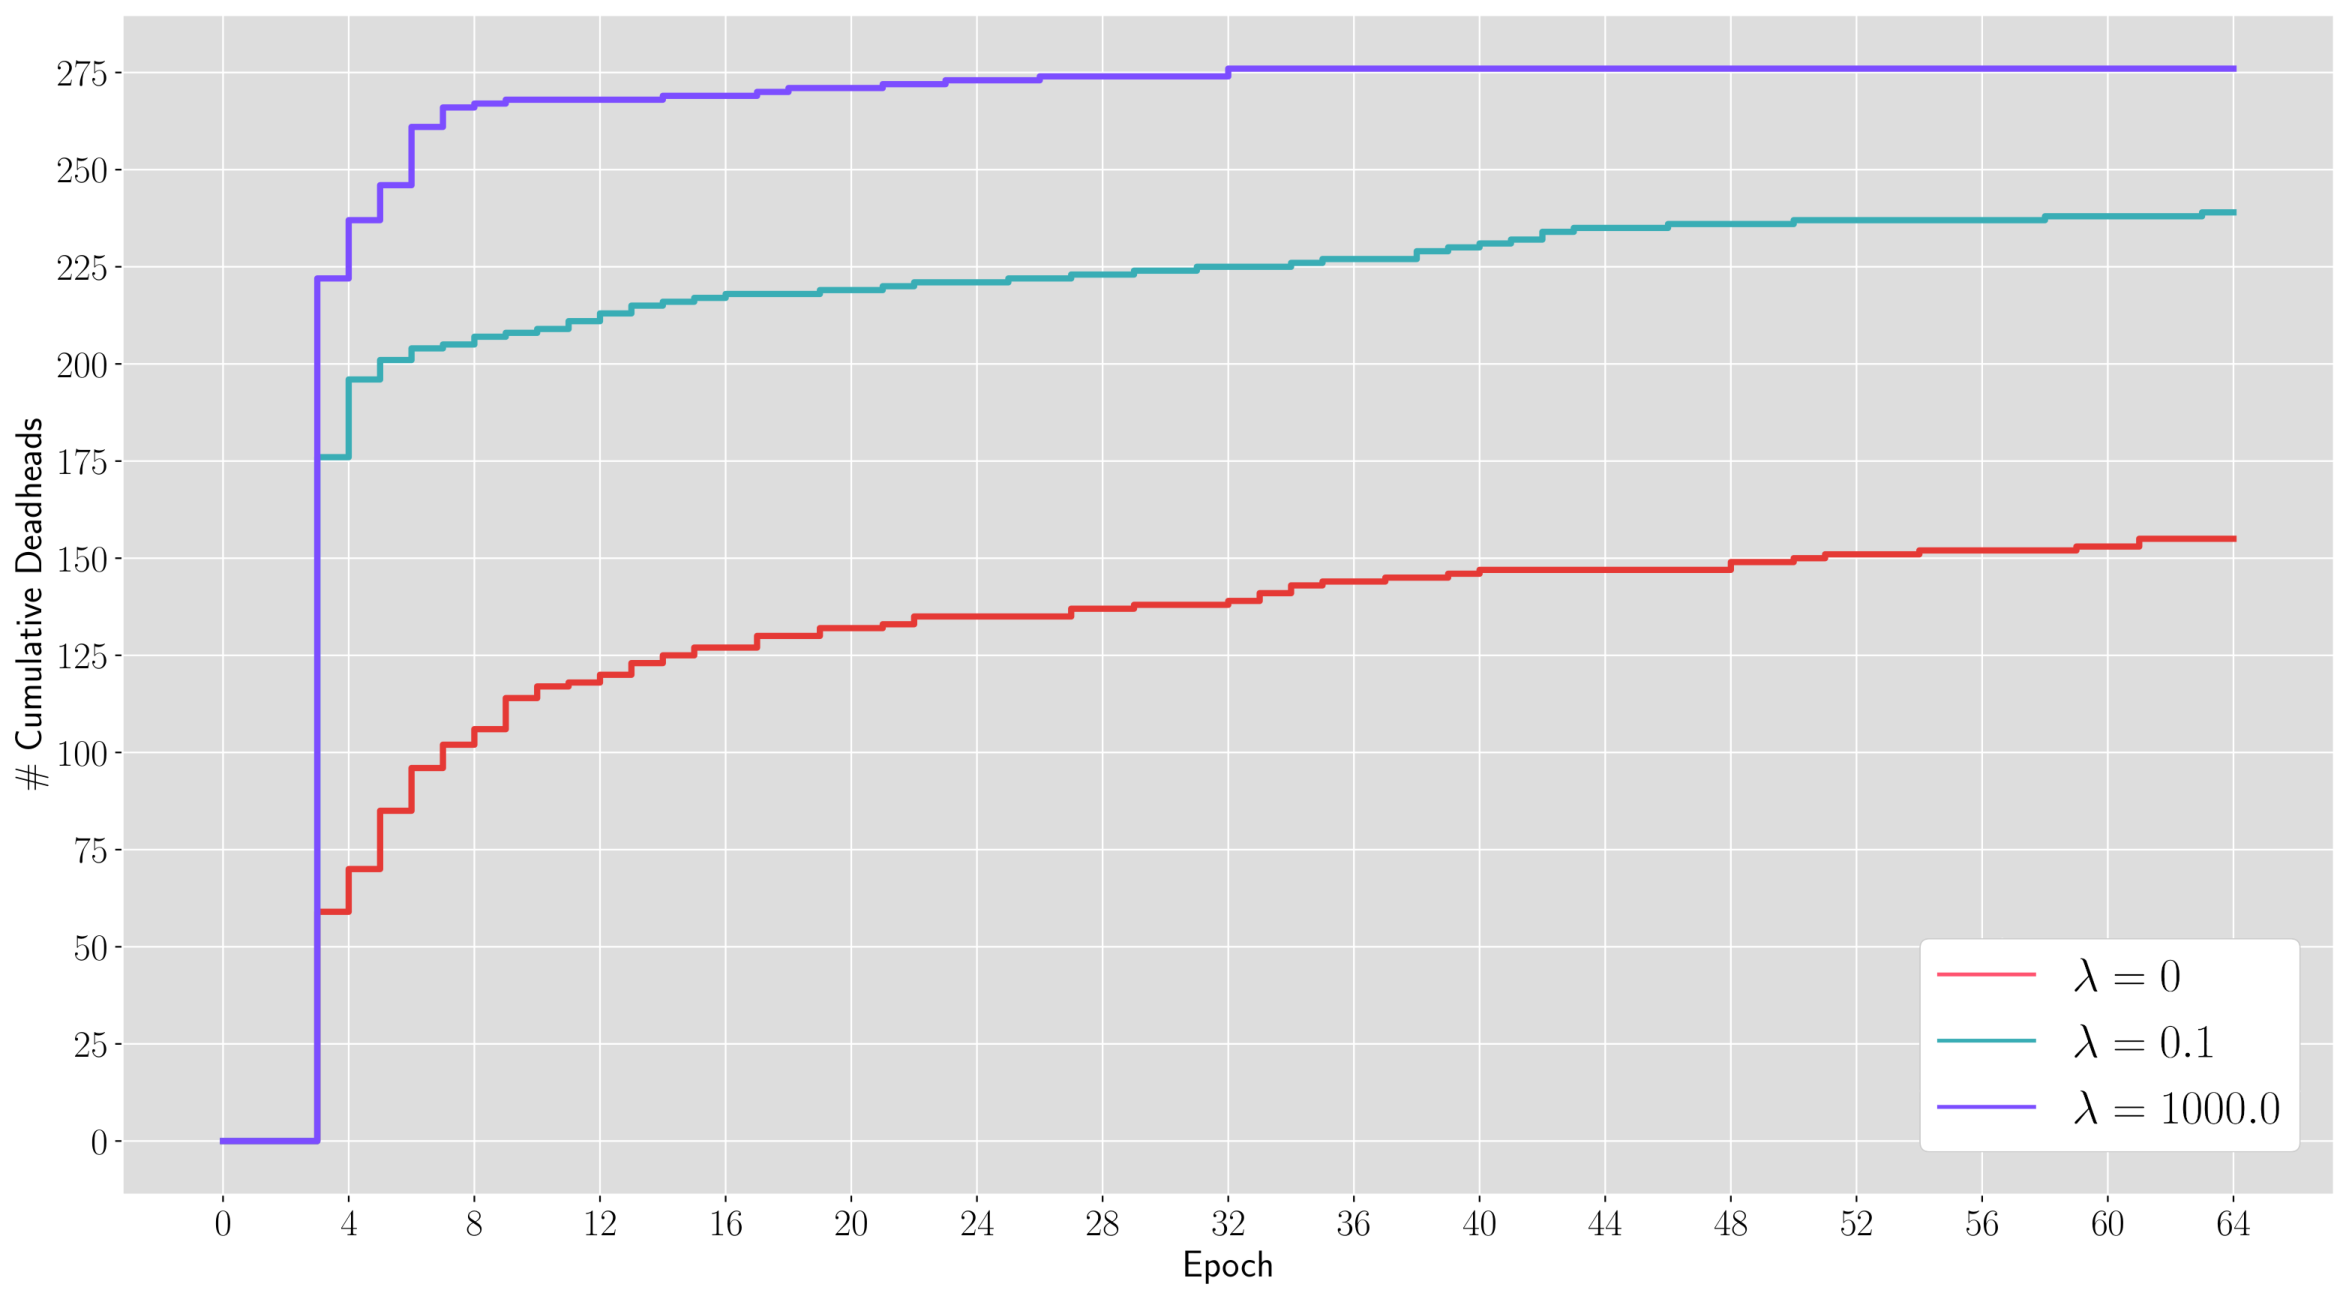
\includegraphics[width=\textwidth]{lambda_exps/deadheads_per_epochLabeled} \\
	\caption[Number of deadheads by epoch for three BonsaiNet models with different $\lambda$ values]{Number of deadheads by epoch for the three models from the $\lambda$ experiments. The deadheading cycle
	for each of these models is 4 epochs, hence the massive spikes at the fourth epoch.}
	\label{fig:deadheads_per_epoch}
\end{figure}

Notice that the most extreme $\lambda=1,000$ model performs 81\% of its total deadheading at the first possible deadheading
opportunity, and 96\% by the third cycle. While not shown in the figure, its soft-compression is even faster: within the first few data
batches it had soft-compressed to the target 0.50 mark. Its lackluster performance suggests that while the aggressive pruning
strategy is good at rapidly performing compression, it lacks the refinement to ensure that this rapid compression is
beneficial in the long-term to its performance. It seems likely that the memory-performance balance of operations evolves over time,
and thus basing all compression on that balance within the first few data batches is short-sighted.

Meanwhile, the $\lambda=0.1$ model achieves similar levels of performance to the free-pruning ($\lambda=0$) model, while still attaining
the goal compression. It also performs a large part (74\%) of its deadheading after the very first cycle,
but the remaining 26\% of the total compression is more gradually distributed over the remaining training epochs.
This is indicative of the approximate balance being sought with the compression $\lambda$; it needs to
motivate enough compression that the model will quickly prune to the correct size, but ensure that
said compression is performed in a careful and prudent manner such that it is not massively detrimental to the potential performance.

A final notable observation from this experiment is that the free-pruning $\lambda=0$ model still compressed by around
27\%; this model found that removing certain internal operations benefited its classification performance, which runs
slightly counter to the general deep-learning intuition that bigger is better. This phenomenon is directly examined in
Section~\ref{sect:supernetevaluation}. The actual decisions being made by the model can be better understood by looking at how frequently certain operations
are chosen across the model, as shown in Figure~\ref{fig:operation_hist}.

\begin{figure}[ht]
    \centering
	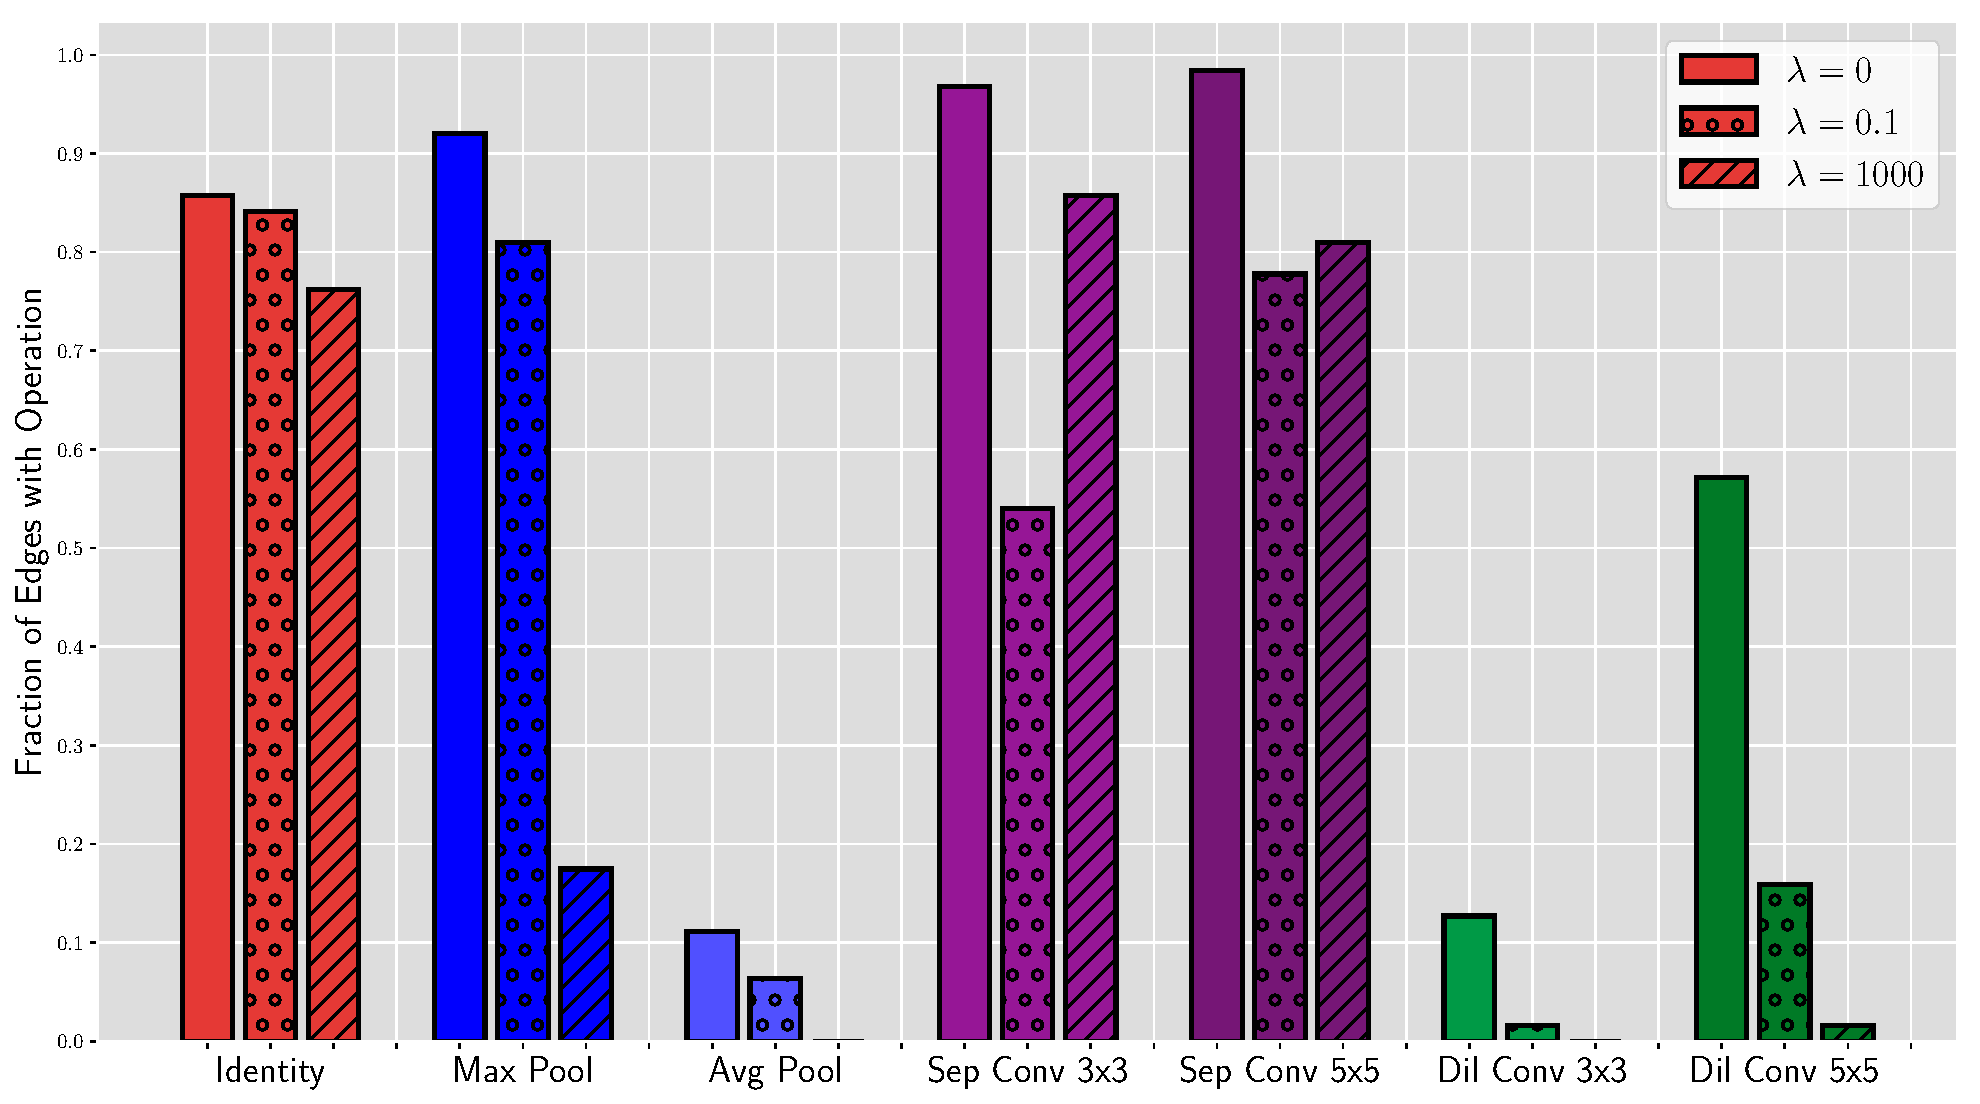
\includegraphics[width=\textwidth]{lambda_exps/joint_operation_spread} \\
	\caption[Operation choices frequencies by $\lambda$ value]{Operation choices by the three models. The y-axis represents the fraction of the edges in the model than
	contain a certain operation. }
	\label{fig:operation_hist}
\end{figure}

Using the freely-pruning model as a reference for the purely task-optimal operation frequencies, notice that
	the $\lambda=0.1$ and $\lambda=1,000$ models vary in behavior
versus the reference. Notably, they make opposite decisions in regard to the max pooling and 3x3 separable convolutions;
the $\lambda=1,000$ model removes the majority of max poolings,
while preserving around 85\% of the 3x3 separable convolutions. The $\lambda=0.1$ keeps 80\% of max poolings, while removing
around half of the 3x3 separable convolutions. Perhaps this was a decision motivated by a tradeoff between memory cost and
the immediate performance gains provided by these operations; remember, the $\lambda=1,000$ soft-compresses near instantly.
In the first few training batches, the model needs to begin moving from some randomly-initialized state towards
a learned optima. This tweaking of weights from completely random to slightly learned in the first epoch is
the largest single-epoch jump in performance that will likely occur in all of training, as there is simply so much
potential performance to gain starting from fully random initialization\footnote{Case in point: the $\lambda=0.1$ model
in its randomly-initialized state has a CIFAR-10 accuracy of 10.00\%. After 1 epoch, its accuracy was 57.20\%, a performance
gain of 47.26 percentage points. The next largest single-epoch performance gain was only 7.64 percentage points.}. The
separable convolutions are immensely powerful in this early training scenario as they have a large amount of
parameters and thus ample room to improve from the random state. Max poolings on the other hand are relatively
memory-expensive (usually exactly half the cost of separable convolutions) but are fixed filters with no learning ability,
and as such do not provide as much immediate power to the model. With this in mind, the behavior of the
$\lambda=1,000$ model can be understood; with only the context of the first few data batches, it removes en masse
the most expensive operation that is providing no immediate advantage over random initialization.

Given the results of these various experiments, it appears that the $\lambda=0.1$ model provides the best compromise between
task performance and pruning.

\subsection{Integrating Pruning} \label{sect:pruner_batchnorm}
With pruners and compression defined, the next step is to integrate them into the architecture. Revisiting the
edge calculation as presented earlier, it computes the sum of the (potentially) pruned output of each candidate
operation:
\begin{align}
	E^{out} = \sum_{i=0}^{\mathcal{|O|}} P^o_i (o_i(E^{in}), w^o_i) \label{eq:candidate_pruner_sum}
\end{align}

\noindent While this looks to accomplish the task set out for pruners; i.e., differentiably select which operations
to keep and which to prune, there is a major issue that arises in practice. This issue is that the output of any such edge
$E^{out}_i$ is the input to every subsequent edge $E^{out}_{i+j}$ in its particular cell. Any learned weights from such
a downstream operation will be learned as a function of that downstream operation's inputs, which are explicitly a function
of the upstream operation configuration. A change to that upstream configuration such as an operation pruner moving from
on to off will add or remove an element from the Equation~\ref{eq:candidate_pruner_sum} sum. This drastically
changes the output distribution of the upstream edge, which in turn is reflected in the input distributions of downstream
operations. When these input distributions are changed, the learned weights of downstream operations are made useless as
they are no longer relevant to the actual tensor values flowing through the operations, the effects of which is highly detrimental
to the loss of the model. As such, changes in operation configuration (and thus changes in pruner state) can cause
	massive spikes in the loss, and are thus highly discouraged in gradient descent.

This exactly mirrors the covariate shift problem described in Section~\ref{sect:batch_norm}. As such, the
exact same solution to the problem as proposed by~\cite{ioffe2015} is applicable: batch normalization. By modifying
the edge calculation as follows:
\begin{align}
	E^{out} = \text{BatchNorm}\left( \sum_{i=0}^{\mathcal{|O|}} P^o_i (op_i(E^{in}), w^o_i) \right) \label{eq:candidate_pruner_sum_bn}
\end{align}

\noindent the operation configuration is decoupled from output distribution. With this calculation, the
`off' pruner state can be thought of not as setting the operation output to zero, but rather to the mean of the edge output distribution.
This way, pruners can experiment with preserving or removing an operation without affecting the input distributions
	of every downstream edge. Furthermore, it
allows models to dynamically prune during training, as operation removal does not affect the relevance of the
model's existing learned weights.

\subsection{Pruning Summary}
With memory compression made possible by the combination of memory-aware pruning and deadheading,
it is now possible to initialize a model and set an arbitrary compression target for it to reach. When the model is trained with
compression loss, computed from the distance between the current compression and the target compression, pruners will
gradually switch off in accordance to however the model sees fit. As pruners remain off for extended periods of time they
will be deadheaded, slowly reducing the model's memory footprint to the desired size. Passing the output of the pruners through
batch normalization ensures that pruning does not shift the output distribution of edges, ensuring that the pruning process
is as non-disruptive as possible to model training. In summary, these components combine to create a method of compressing an arbitrary model
to a specific VRAM size in a way that is minimally detrimental to the performance of said model.

\section{Cell Search}~\label{sect:bonsai_cell_search}
To solve the problem of searching for unique cells via a supernet technique, an iterative stacking approach was chosen.
To do this, a virtual supernet is created consisting of however many cells is desired. This supernet is then divided into
\textit{model sections}, groups of consecutive cells within the model,
	such that each section is roughly the same size and the first section
	can fit into a specified max VRAM footprint $s_{max}$ in the fully superconnected state. This max VRAM footprint is often the currently
available free space on the GPU VRAM, but could also refer to the space on the desired deployment hardware or
simply the desired final size of the model.

\vspace{2em}
\noindent To concisely and specifically describe the cell search process, the following notations are defined:
\begin{definition}
	A model section is a group of consecutive cells, such that each section is roughly the same size. For example,
	a model with nine cells might be comprised of three sections of three cells each: $[C_0, C_1, C_2]$, $[C_3, C_4,C_5]$, and $[C_6,C_7,C_8]$
\end{definition}
\begin{definition}
	To describe a composition of model sections that form a larger model:
	\begin{align}
		M^{[0,1,\dots,n]}_{[\hardcomp,\hardcomp_1,\dots\hardcomp_n]} = M^0_{\hardcomp_0} + M^1_{\hardcomp_1} + \dots + M^n_{\hardcomp_n}
	\end{align}

	\noindent Here, $M^i_{\hardcomp_i}$ refers to the $i$th model section hard-compressed to some level $\hardcomp_i$, while
	$M^{[0,1,\dots,n]}_{[\hardcomp_0,\hardcomp_1,\dots,\hardcomp_n]}$ refers to a model comprised of sections 0 through n, each hard-compressed to a level
	$\hardcomp_0$ through $\hardcomp_n$, respectively. Using this notation, a section $i$ in the superconnected state would be written as
	$M^i_1$, while a fully compressed section (i.e., empty) would be written as $M^i_0$. The notation $M^0_{\hardcomp_0} + M^1_{\hardcomp_1}$
	indicates appending section $M^1_{\hardcomp_1}$ after $M^0_{\hardcomp_0}$, such as to combine them into one contiguous graph $M^{[0,1]}_{[\hardcomp_0, \hardcomp_1]}$. This
	operation is shown graphically in Appendix~\ref{chapter:bonsai_architectures}, Figure~\ref{fig:bonsai_growth}.
\end{definition} \label{def:model_sections}


\begin{definition}
	The $i$th \textit{subset} of $M$ refers to a model $M^{[0,1,\dots,i]}_{[\hardcomp_0,\hardcomp_1,\dots,\hardcomp_i]}$,
	where $i$ is less than the total number of sections in the full model $M$.
\end{definition}


To perform cell search using this stacking, first the initial section $M^0_1$ is loaded onto the GPU. A classification tower
is added after this section, such that $M^0_1$ can be treated as a fully functional standalone model; the $0$th subset of
$M$. $M^0_1$ is then trained and
pruned until enough space is freed such that section $M^1_1$ can be appended to the model. The model, the first subset of $M$, is now:
\begin{align}
M^{[0,1]}_{[\hardcomp_0,1]} = M^{0}_{\hardcomp_0} + M^{1}_{1}
\end{align}

\noindent The existing classification tower is then converted to an auxiliary tower, and a new classification tower is added
after section 1. This extracts further benefit from the old classification tower; while technically no longer necessary,
auxiliary towers help regularize a model as described in~\cite{szegedy2014}.  This growing and pruning process is then
cycled until the final section can be added, and the model is:
\begin{align}
M^{[0,1,..,n-1,n]}_{[\hardcomp_0,\hardcomp_1,\dots,\hardcomp_{n-1},1]} =  M^{0}_{\hardcomp_0} +  M^{1}_{\hardcomp_1} + \dots + M^{n-1}_{\hardcomp_{n-1}} + M^{n}_{1}
\end{align}

See Appendix~\ref{chapter:bonsai_architectures}, Figure~\ref{fig:bonsai_growth} for a graphical representation
of this growth process and its effect on the model's connectivity.

At this point, all sections 0 through $n-1$ have compressed to some $\hardcomp_0$ though $\hardcomp_{n-1}$; each of these sections
is now ideally at the optimal architecture for its respective compression level.  However, in order for this process
to be feasible, the space requirements of each section must be established, such that
a) the compression target for that section of the model is known and b) when there is enough free space
to stop compressing and add the next section. This is to say, it is necessary to know the largest $\hardcomp_0, \dots, \hardcomp_i$ such that
$M^{0,1,\dots,i}_{\hardcomp_0, \dots, \hardcomp_i} +  M^{i+1}_{1}$ fits into the desired VRAM footprint. To do this, there needs to be an accurate
estimate of the VRAM size of the $ith$ model subset.


\subsection{Operation and Model Size Estimation} \label{sect:operation_sizing}
 In order to test whether some model subset $M$ at a specific hard-compression level $\hardcomp$ will fit into $s_{max}$, a
\textit{simulation model} is used. A simulation model is simply some model $M'$ that has an identical structure to $M$,
that is, one with identical number of cells, edges, and edge connectivities. However, at initialization, $M'$ has
no operations along any of the edges. The simulation model $M'$ is then filled with operations until it
reaches $\hardcomp$, at which point its size can be measured to check fit.

The problem of filling the model with operations can be modeled as a change-making problem~\citep{wright1975},
where a certain number of operations are picked such that the overall compression of the model is as close
as possible to the target compression. In order to perform this accurately, an accurate estimate of the size of
each operation is needed, that is, the amount of VRAM used by this specific operation within the model. Ideally, it should be
an additive operation size estimate, one such that the sum of the sizes of all component operations is equal
to the total size of the model.

To do this, five factors need to be considered. First is the allocation required by the operation itself, that is, the space
needed to store the weights of the operation and the pruner. Second is the allocation required to perform forward and
backward computation of the operation, which requires storage of output, intermediate, and gradient tensors. Third is
the the size consequences of interaction effects between operations. Namely, as each
operation arrives in a node, it must be summed together with the other inbound operations. Therefore, each operation
except for the very first into a node incurs a summation operation, which results in a tensor allocation. That means that in the most
common case (where an operation is not the first operation to arrive at a node) this extra summation and therefore
tensor allocation occurs. Fourth, the ``warmup'' effects displayed by certain operations must be accounted for; certain
operations will allocate a certain amount of memory for their first computational pass, then ask for slightly more in the
second. After the second computation, their allocation remains fixed at the new, higher level. This extra allocation
comes from operations that contain batch normalizations which require tensor space to store
statistics from the current and previous batches, the latter of which is unnecessary for the very first batch. Finally,
the non-monotonic allocational behavior of PyTorch must be measured. The exact space used by an operation can rapidly
fluctuate throughout the process of its computation as tensors are allocated and deleted as needed. PyTorch will allocate space
according to the maximum allocation that occurs during an operation's lifespan;
regardless of whether this maximum is a transient peak, it nevertheless sets the permanent allocational size of the
operation and whether an out-of-memory error occurs.

The algorithm used to
estimate the size of operations within BonsaiNet models is given in Algorithm~\ref{alg:revised_operation_sizing}:
\begin{algorithm}
	\nl let $\mathcal{M}$ refer to measuring the current Torch memory allocation\;
	\nl let $n_{repetitions}$ refer to the number of measurements to average/summarize over\;
	\nl $m = 0$\;
	\For{$0 \to n_{repetitions}$} {
		\nl $\mathbf{m} = \varnothing$\;
		\lnl{size:meas0} $m_{pre} = \mathcal{M}$\;
		\lnl{size:init} Initialize operation $o$ and pruner $p$\;
		\For{$0 \to n_{repetitions}$} {
			\lnl{size:meas1} $\mathbf{m} = \mathbf{m} \bigcup (\mathcal{M} - m_{pre})$\;
			\lnl{size:forward} Pass sample input of dimensionality $d$ \textit{forwards} through $o$ and $p$, store output\;
			\lnl{size:meas2}  $\mathbf{m} = \mathbf{m} \bigcup (\mathcal{M} - m_{pre})$\;
			\lnl{size:interaction} Add output to itself\;
			\lnl{size:meas3} $\mathbf{m} = \mathbf{m} \bigcup (\mathcal{M} - m_{pre})$\;
			\lnl{size:backwards1} Pass output through sample loss function\;
			\lnl{size:meas4}  $\mathbf{m} = \mathbf{m} \bigcup (\mathcal{M} - m_{pre})$\;
			\lnl{size:backwards2} Pass gradient \textit{backwards} through $o$ and $p$\;
		}
		\lnl{size:peak} $m = m + \max(\mathbf{m})$
	}
	\KwResult{$\frac{m}{n}$}
	\caption{Compensated Operation Sizing}
	\label{alg:revised_operation_sizing}
\end{algorithm}

The algorithm first makes note of the current GPU allocation (Line~\ref{size:meas0}) prior to the start of size estimation.
Line~\ref{size:init} initializes an identical operation and pruner to the estimated operation, thus ensuring that the
allocation of the operations themselves are measured. Line~\ref{size:forward} measures the allocational requirements
of the forwards pass of the operation, while lines~\ref{size:backwards1} and~\ref{size:backwards2}  measure the backwards pass.
Line~\ref{size:interaction} sums
the output of the estimated operation with itself, and thus simulates the allocational interaction effects that
would occur in node summations of the real model. The forwards-backwards passes are repeated $n_{repetitions}$ times (typically 5),
to account for potential warmup effects. After each step of the algorithm, the current memory allocation is
compared to the initial allocation (lines~\ref{size:meas1},~\ref{size:meas2},~\ref{size:meas3}, and~\ref{size:meas4}).
This allows Line~\ref{size:peak} to measure the size of the largest allocational peak, and thus account for the potentially
non-monotonic allocation throughout the calculation of the operation. This largest allocation peak is stored as the
allocation requirement for this specific simulation in line~\ref{size:peak}. Finally, $n$ total of these simulations
are run, and the average allocation requirement over the $n_{repetitions}$ simulations is returned as the estimated size of the operation.

With a hopefully accurate and additive operation size estimate (both these assumptions to be evaluated later in this section),
it is possible to design a method of packing the simulation model $M'$ to the target compression level. To do this, the problem is approached one cell at a time, with each cell allocated
operations independently of one another. For each cell $C$ and for each operation dimensionality $d$ with that cell,
the set of operations $\mathcal{O}_{C,d}$ within is collected. Since the operation size estimation is ideally an additive one,
this means the total size of that set of operations can be easily estimated as the sum of the estimated size of each operation:
\newcommand{\size}{\text{size}}
\begin{align}
	\size(\mathcal{O}_{C,d}) = \sum_{o \in \mathcal{O}_{C,d}}{\size(o)} \label{eq:additive sizing}
\end{align}
The total size of the cell is therefore:
\begin{align}
	\size(C) = \sum_{d \in C} \; \sum_{o \in \mathcal{O}_{C,d}}{\size(o)}
\end{align}
To find the allocational size of the cell that gives the desired compression, the cell size is multiplied by
$c_{tgt}$. By the distributive property:
\begin{align}
	s_{tgt} = c_{tgt} * \sum_{d \in C} \; \sum_{o \in \mathcal{O}_{C,d}}{\size(o)} \\
	s_{tgt} = \sum_{d \in C} \; c_{tgt} \sum_{o \in \mathcal{O}_{C,d}}{\size(o)}
\end{align}
This means that the allocational problem can be reduced to finding the set of operations
$\mathcal{O}' \subset \mathcal{O}_{C,d}$ such that $\size(\mathcal{O}')=c_{tgt} * \size(\mathcal{O}_{C,d})$ for all
$C, d$ within the model. This can be accomplished by using a greedy change-making algorithm, that selects operations for
the chosen subset according to some heuristic over the available operations. In the process of designing this algorithm
three different heuristics were compared: maximum, random, and minimum selection. All three heuristics create a set of available operations $\mathcal{O}_{avail}$,
which contains all unselected operations
that can be added to $\mathcal{O}'$ without increasing its total size above the target. The maximum heuristic then selects
the largest operation within $\mathcal{O}_{avail}$ to be added to $\mathcal{O}'$, the minimum selects the smallest, and
the random selects an operation at random. These heuristics were chosen
based on solutions to the change-making problem as described in \hyperlink{cite.martello1980}{``Optimal and
Canonical Solutions of the Change Making Problem''},~\cite{martello1980}. Specifically, the maximum heuristic matches
\citeauthor{martello1980}'s `canonical solution', designed to find a solution with approximately the minimum number of
operations possible. The minimum heuristic is designed to do the opposite, to approximate a solution with the maximum number of
operations, while the random heuristic should find solutions that lie somewhere in the middle.
Once the heuristic selects an operation, it is added to $\mathcal{O}'$, and the algorithm repeats.
Once there are no more operations that are eligible for $\mathcal{O}_{avail}$, the $\mathcal{O}'$ is fully allocated and the
algorithm ends. This process is detailed in full in Algorithm~\ref{alg:operation packing}.

\begin{algorithm}
	\SetAlgoLined
	let $\mathcal{O}'_{M'}$ be the set of chosen model operations, $\mathcal{O}'_{M'} = \varnothing$\;
	let $s_{current} = 0$\;
	\For{\upshape cell $C \in M'$} {
		\For{\upshape operation dimension $d \in \; C$} {
			let $\mathcal{O}_{C,d}$ equal the set of all operations in $c$ with dimension $d$\;
			let $\mathcal{O}'$ be the set of chosen cell operations, $\mathcal{O}' = \varnothing$ \;
			\lnl{sim model:size target} let $s_{tgt} = c_{tgt} \left( \sum_{o \in \mathcal{O}_{C,d}}{\size(o)} \right)$ \;
			\While{$s_{current} < s_{tgt}$} {
				let $s_{min}$ be the size of the smallest operation available, $\min_{o \in \mathcal{O}_d} \size(o)$\;
				\eIf{$s_{min}+s_{current} > s_{tgt}$ or $\mathcal{O}_{C,d} \setminus \mathcal{O}'=\varnothing$}{
					break;
				}{
					\lnl{sim model:min avail} let $\mathcal{O}_{avail} = \{ o | o \in \mathcal{O}_{C,d} \setminus \mathcal{O}', \quad s_{current} + \size(o) \le s_{tgt} \}$\;
					Choose $o_{chosen}$ from $\mathcal{O}_{avail}$ according to some heuristic $H(\mathcal{O}_{avail})$\;
					$\mathcal{O}' = \mathcal{O}' \cup \{o_{chosen}\}$\;
					$\mathcal{O}_{C,d} = \mathcal{O}_{C,d} \setminus \{o_{chosen}\}$\;
					\lnl{sim model:size addition} $s_{current} = s_{current} + \size(o_{chosen})$\;
				}
			}
			$\mathcal{O}'_{M'} = \mathcal{O}'_{M'} \cup \mathcal{O}'$\;
		}
	}
	\caption{Operation Allocation}
	\label{alg:operation packing}
\end{algorithm}


The rationale for evaluating different heuristics of operation selection is to determine the accuracy of the
operation size algorithm as well as evaluate how well it aligns with the desired additive property. The three heuristics
build models of varying operation counts; the maximum heuristic builds models with minimal operation counts, the minimum
heuristic with maximal operation counts, and the random somewhere in the middle. If the size estimation algorithm is
accurate and additive, any model produced by Algorithm~\ref{alg:operation packing} should be very close to $s_{tgt}$ in size,
and thus should have compression close to $c_{tgt}$, regardless of operation count and therefore selection heuristic.
If the sizing algorithm is inaccurate or non-additive, the calculations in Algorithm~\ref{alg:operation packing} that
rely on said sizing (lines marked~\ref{sim model:size target},~\ref{sim model:min avail}, and~\ref{sim model:size addition})
will be similarly inaccurate. Chiefly, line~\ref{sim model:size addition} is crucial in determining the stopping point of
the algorithm, and as such any inaccuracy will produce models that miss $s_{tgt}$ or $c_{tgt}$. High operation count
models like those produced by the minimum heuristic would increase the number of times these summation inaccuracies might
occur, and thus produce models of differing $s_{tgt}$ or $c_{tgt}$ as compared to the other heuristics. The results of
operation selection across the three heuristics are shown in Figure~\ref{fig:changemaking}.

\begin{figure}[ht!]
    \centering
	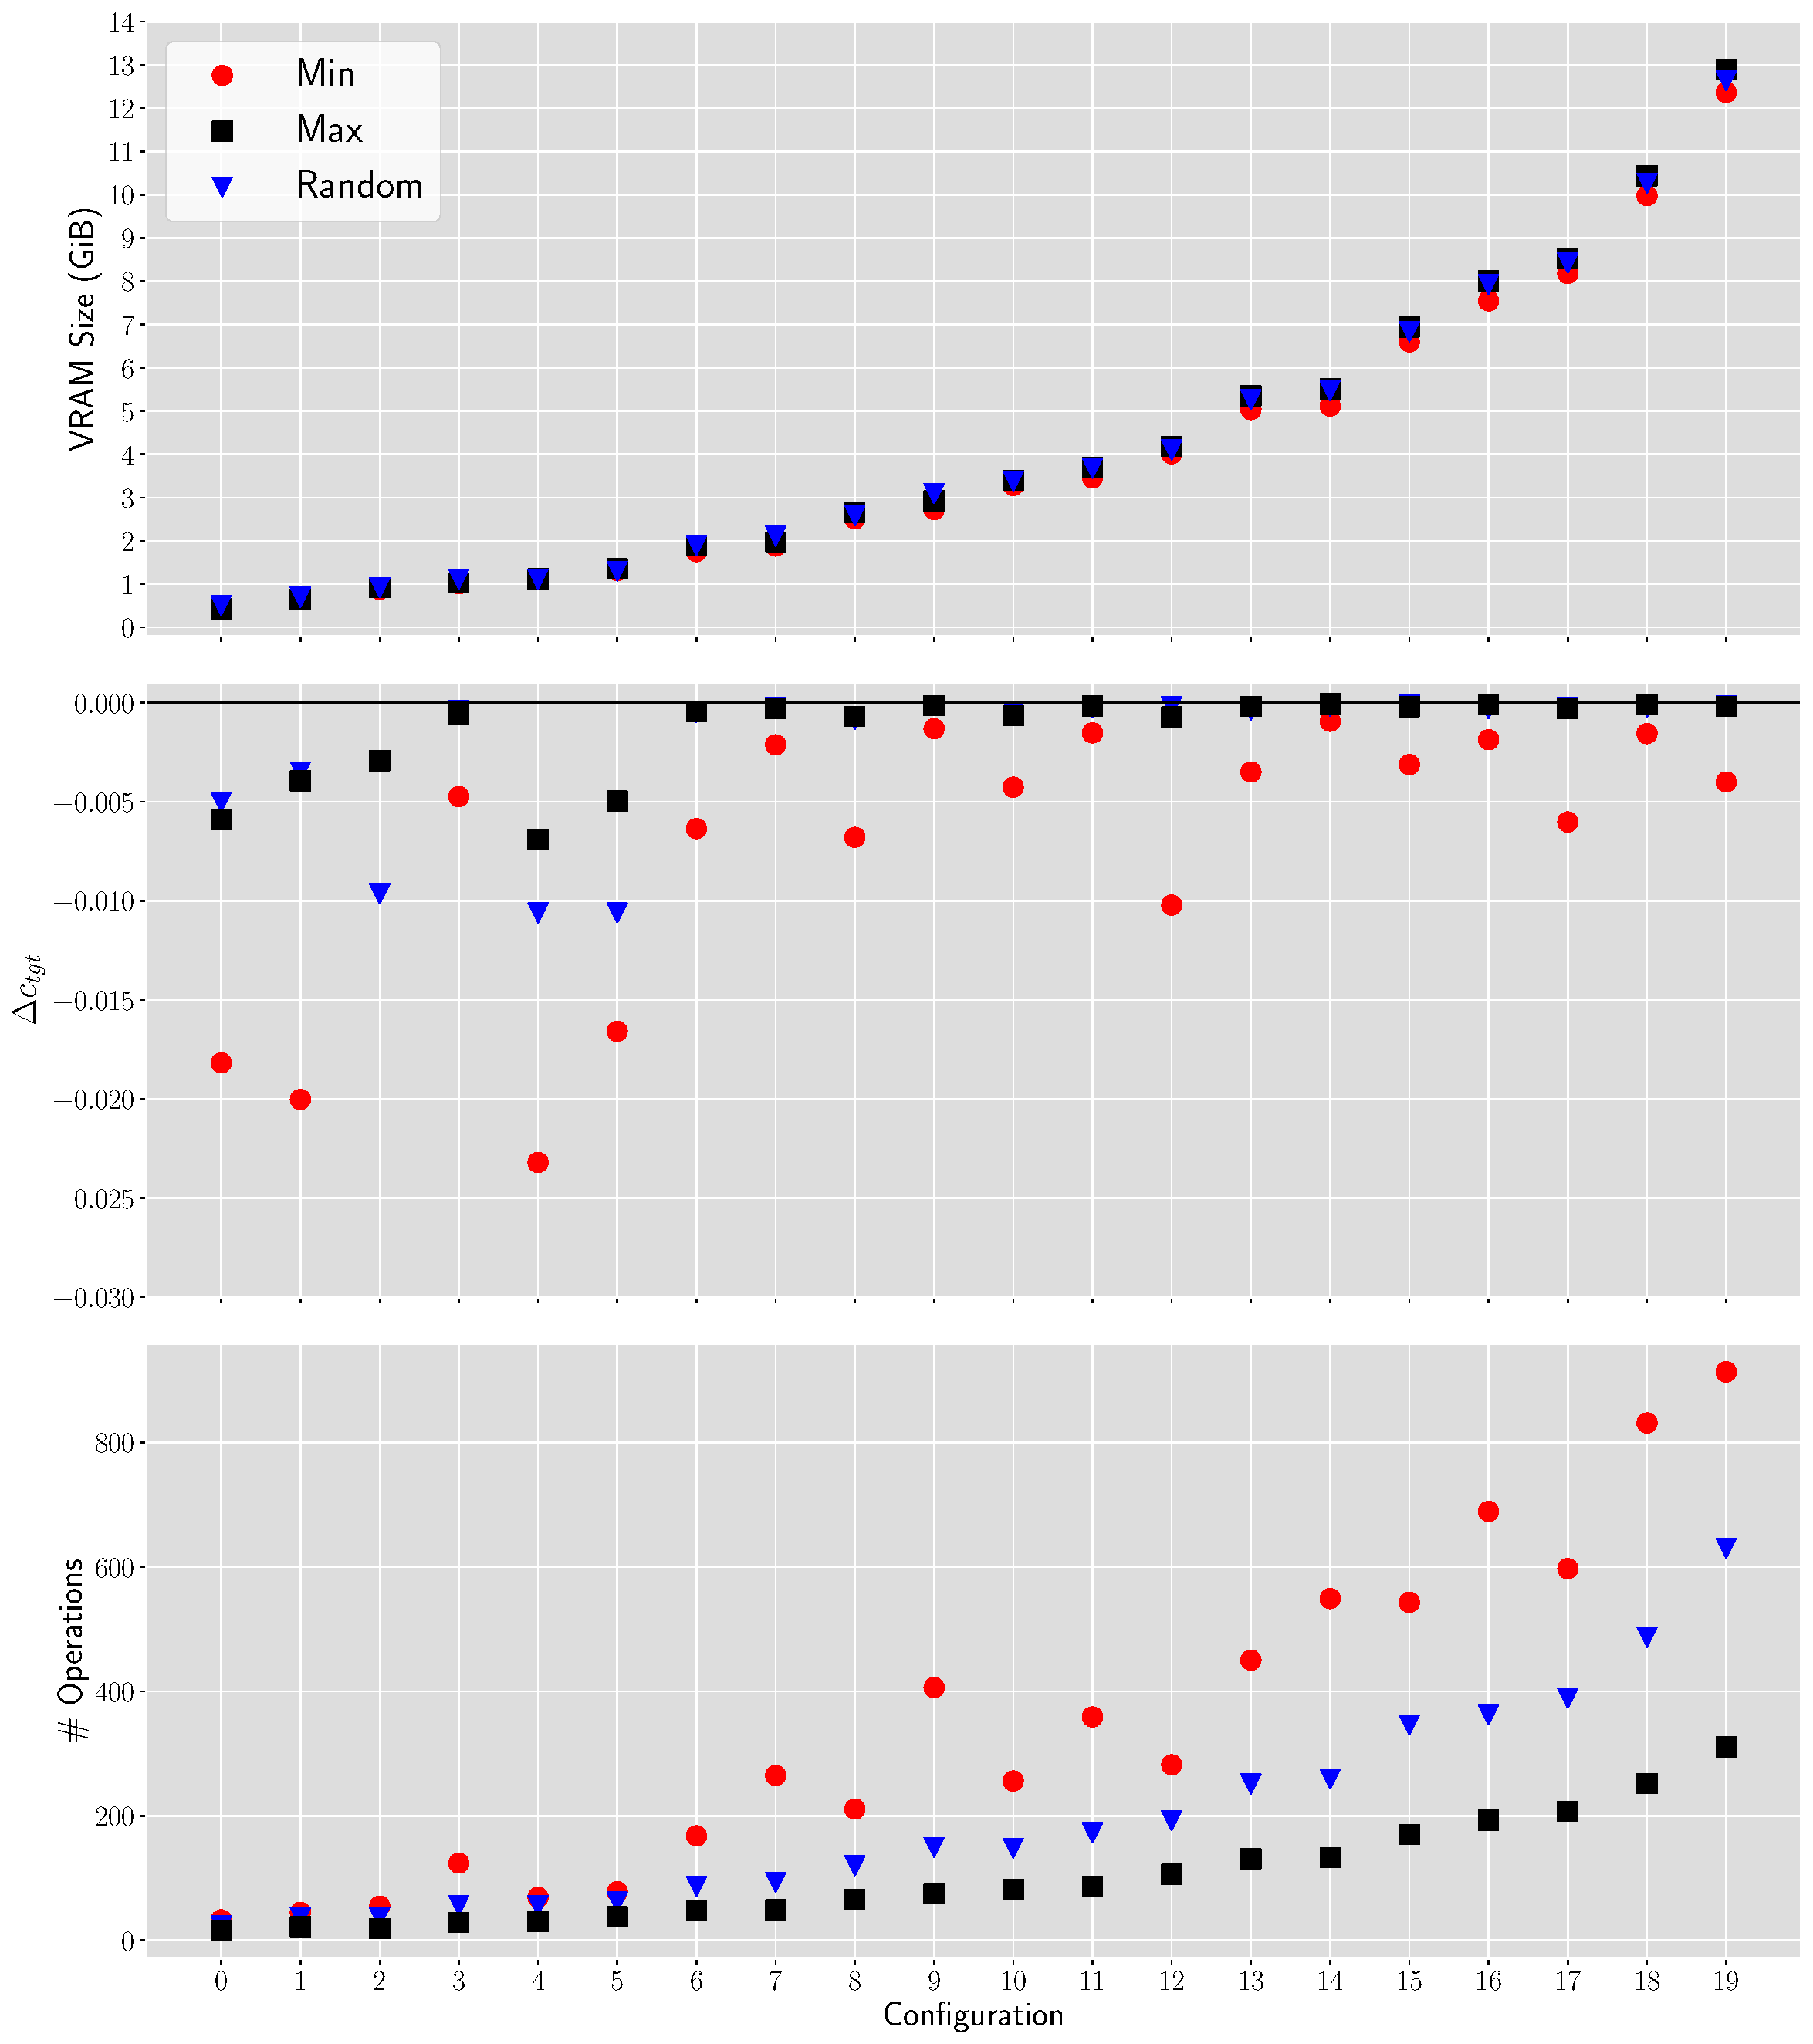
\includegraphics[width=\linewidth]{binpacking} \\
	\caption[Comparison of three different operation selection heuristics within the greedy change-making algorithm]{Comparison of three different operation selection heuristics within the greedy-change making algorithm.
	60 models were allocated in total, corresponding to 20 different model specifications each allocated operations by three
	heuristics.	Shown are the VRAM size (top),  difference between target compression
	and allocated compression (middle), and number of operations (bottom) plotted against configuration and heuristic.}
	\label{fig:changemaking}
\end{figure}

To evaluate this, 20 different model configurations are packed according to the three heuristics and measure the resulting model's
VRAM size, delta to compression target, and operation count. To measure the VRAM size of any particular model, the
 VRAM allocation prior to the model's initialization is first noted. Then the model is moved onto the GPU, and the
VRAM allocation after passing two full data batches through the model both forwards and backwards is measured.
Two batches are necessary for accurate size measurement due to the same allocational ``warmup'' condition as described earlier.
To avoid potential stuck-tensor issues if the simulation model encounters an out-of-memory error, simulation models
 are initialized in a subprocess forked from the main process. This means there is a separate Torch context initialized in
the subprocess, which means that all tensors initialized in the subprocess are compartmentalized from those in the
main process. If the subprocess simulation model encounters an out-of-memory error, the process returns a failing exit
code and terminates. When the subprocess terminates, its Torch context deletes and garbage collects all tensors
that were initialized within it, cleaning any potentially orphaned tensors off the GPU.
Essentially, the subprocess sandboxes the simulations from the main process, meaning size testing can occur without
worrying about destroying the viability of the main process.

Notice that the three heuristics do indeed
produce models that are consistently ranked in terms of operation count (bottom plot); the maximum heuristic chooses the fewest operations,
followed by random, and minimum chooses the most. Despite this, the VRAM size of the models are highly consistent despite
the operation count disparities, meaning that maximum heuristic is choosing a few large operations, while the minimum is
choosing many small operations\footnote{One thing to note is the minimum heuristic's consistent inability to fully reach $c_{tgt}$.
This is because solutions to the change making problem assume an infinite number of available choices at each size, whereas in this case
there are a finite number of operations to select. The minimum heuristic, by way of trying to select maximum operations,
sometimes runs out of available operations before it can satisfactorily produce a model of size $s_{tgt}$.}.
Overall, the sizing demonstrates the exact behavior hoped for: the operation size estimator is accurate and additive,
and that the compression of models is an accurate indicator of its VRAM size.

In conclusion, Algorithm~\ref{alg:revised_operation_sizing} provides accurate and additive operation size estimates,
which allows Algorithm~\ref{alg:operation packing} to accurately produce simulation models $M'$ of an arbitrary compression
level. This in turn checks whether a model of that compression level will fit into VRAM.
This is tremendously useful for this use-case because there is no way of providing any guarantee about a model's
real-world connectivity and operation count as it prunes to a certain compression level. It might prefer a small or large
operation count, meaning that the way that is achieves that specific compression is highly dependent on its individual
circumstances. With accurate sizing, it is possible to know for sure that any model at a particular compression will fit if the
simulation model does.

\subsection{Compression Targets}
With a reliable method of checking whether an arbitrary model subset at a specific compression
will fit into the desired amount of VRAM, the compression targets for each section of the model can be set. This is
approached from an inverse perspective; rather than estimate the size $s_M$ of a model subset
and setting the compression target $c_{tgt}$ as $\frac{s_{max}}{s_M}$, instead the largest compression level is found such that
subset plus the new section fits into a given maximum VRAM allocation $s_{max}$:
\begin{align}
c_{tgt_i} = \max \{ c \in [0, 1] \; | \; \text{size}(M^{0,\dots,i-1}_{\hardcomp_0, \dots, \hardcomp_{i-1}} + M^i_1) \le s_{max} \}, \label{eq:comp_target}
\end{align}

Since the process of testing a particular simulation model size involves model initializing, operation packing,
GPU transfer, and a couple of data passes, it is relatively slow; usually on the order of a couple of seconds per test.
This means the total number of size tests needs to be minimized. To search the compression space (the $c \in [0, 1]$ term
from Equation~\ref{eq:comp_target}) efficiently, a binary search tree is traversed, as per Algorithm~\ref{alg:bst}:

\begin{algorithm}
	\SetAlgoLined
	let $c_{tgt}=[0, 0, \dots, 0]$\;
	let $d$ be the maximum depth of the search tree to search
	\For{$n_{section} \in [0, \# sections]$}{
		let $c=0.5$\;
		let $\Delta=0.25$\;
		\For{$i \in [0,d]$} {
			\eIf{\upshape $\text{size}(M^{0,\dots,i-1}_{c} + M^i_1) \le s_{max}$}{
				$c_{tgt_i} = c$\;
				$c = c + \Delta$\;
			}{
				$c = c - \Delta$\;
			}

			Reduce step size unless at final step (this allows c=0 and c=1 to be attainable)\;
			\If{$\Delta > 2^{-depth-1}$}{
				$\Delta = \Delta/2$\;
			}
		}
	}
	\caption{Compression Target Search}
	\label{alg:bst}
\end{algorithm}

\noindent The depth parameter $d$ of the search tree controls the search granularity: the finest increments that can be searched by
the algorithm. For the purposes of BonsaiNet, the depth was set to 6 as it provides a search granularity of $\frac{1}{2^6} \approx 0.015$,
meaning that the space between 0 and 1 is searched in increments of $0.015$. This therefore sets the upper bound at the
possible error in the compression target search algorithm, as the distance between the optimal compression target and the
one returned by the algorithm will be at most $0.015$. In a future implementation, the optimal search depth could also be
automatically calculated from the model configuration:
\begin{align}
	\text{depth} = \lceil \log_2 \frac{\sum_{o \in M} \text{size}(o)}{\min_{o \in M} \text{size}(o)} \rceil,
\end{align}
\noindent where $sum_{o \in M}$ iterates over each operation $o$ in the model. Compression is implicitly a discrete metric, where the smallest
quanta is determined by the smallest operation within the model. The above equation would guarantee that the search
granularity is always marginally finer than the compression difference created by toggling on or off the smallest operation in the model.

This algorithm provides us with $c_{tgt}$ values for each section of the model. However, these targets represent
the compression levels that are at the absolute extreme of what can fit into the desired VRAM footprint; the search
depth of 6 means that while $c_{tgt}$ might fit, $c_{tgt}+0.015$ will not. As such, it is absolutely crucial that the models
arrive underneath these targets, simply to guard against out-of-memory errors and the stuck tensors issues they cause.
However, there is an even larger issue with passing these compression targets to the loss function, and that is due to the
means by which compression loss computes $\mathcal{L}_{comp}$. As seen in equation~\ref{eq:comp_term_vector},
the $\mathcal{L}_{comp}$ is proportional to the square distance of the actual compression to the target compression. This means that
as the model approaches the target compression, $\mathcal{L}_{comp}$ falls exponentially, thus exponentially slowing further
progress to the target. This initiates a negative feedback loop, eventually halting all progress at compression level
marginally above the target. Therefore, in order to actually meet the compression targets the model needs to aim to
overshoot them. To do this, define:
\begin{align}
	\softcomp_{aim} &= \begin{cases}
		0.90c_{tgt}, & c_{tgt} > 0.35\\
		0.66c_{tgt}, & c_{tgt} \le 0.35
	\end{cases} \label{eq:c_aim}
\end{align}
\noindent And redefine:
\begin{align}
	\mathcal{L}_{comp} &=  ||\mathbf{\softcomp} - \softcomp_{aim}|| \label{eq:comp_aim_term_vector}
\end{align}

\noindent This establishes an overshoot $\softcomp_{aim}$ that is marginally smaller than $c_{tgt}$, with the margin varying by
the size of $c_{tgt}$. The larger margin at compression levels below $0.35$ is experimentally motivated; compressing down
below that size tends to incur significant task performance penalties, which highly disincentivizes the model performing
significant compression in those regions. Increasing the overshoot here effectively increases the weight of the compression
penalty term as compared to the task performance loss, in an attempt to rebalance the two and motivate compression in
high-compression domains.

There are now two different compression targets $c_{tgt}$ and $\softcomp_{aim}$ that arise from Algorithm~\ref{alg:bst} and Equation~\ref{eq:c_aim}
respectively. $c_{tgt}$ is a physical hardware constraint: it refers to the biggest the model can possibly be to avoid
exceeding the VRAM allocation restriction $s_{max}$. As such, this corresponds to the hard-compression of the model: the
compression produced by the permanent deletion of deadheading operations from the model. However, hard-compression
must lag behind soft-compression, as deadheading can only occur when an operation has been consistently turned off. This
is to say the hard-compression of an operation can only occur after it has been consistently soft-compressed, which therefore
lags the two metrics. By setting $\softcomp_{aim}$ to be proportionally smaller that $c_{tgt}$, this lag can be compensated for
such that when the soft-compression $\softcomp$ reaches $\softcomp_{aim}$, the hard-compression $\hardcomp$ reaches $c_{tgt}$.

\subsection{Breaking Codependence} \label{sect:breaking codependence}
While training a model with the adjusted $\softcomp_{aim}$ compression target ensures that the model will eventually reach a
compression level below $c_{tgt}$ if sufficiently motivated to do so, often the speed of compression will slow significantly
after the first deadheading cycle. If left unchecked, compression will eventually come to almost a complete halt, which
prevents a model from reaching $c_{tgt}$ if it starts sufficiently far from the target. This can be easily demonstrated
by looking at the number of deadheads per epoch for each of the three example models from Section~\ref{sect:lambda_choice},
and the plateauing compression is shown in Figure~\ref{fig:deadheads_per_epoch}.

Notice that the number of deadheads per epoch scales with the $\lambda$ value, but trails off significantly in each model
after the first 12 or so epochs. This slowing is due to two main reasons. First, the compression loss scales with the
square of distance, so as the model gets closer to the aim, the rate at which it slows decreases correspondingly. The second
reason is codependence as described in Section~\ref{sect:pruner_batchnorm}, where operations' weights will become more dependent on each
other the longer they remain jointly active. This demotivates compression, as any removed operation will negatively affect
any and all codependent operations. While the presence of batch normalizations along edge outputs mitigates these effects
to some degree, they can only ensure that edge outputs
lie within a consistent overall distribution, not that the content of that output aligns with what is expected by downstream
operations.

There are three ways to try to avoid or break this codependence. The first way, and the easiest, is to ensure that
the model configuration is such that none of the $c_{tgt}$ values of any model subsection are particularly challenging. As
seen in Table~\ref{tab:lambda_comparisons}, models will naturally compress to levels around $0.70$, and have no trouble
getting down to $0.50$. Beyond around $0.40$, however, and models start taking quite a long time reaching targets due to
the aforementioned slowing factors. By simply ensuring that the configuration avoids such values this problem is circumvented,
which can be accomplished by strategies like reducing the number of operations per edge or nodes per cell.

Second, the slowing compression can be countered by increasing
the compression penalty over time. Here, the $\lambda$ value is doubled after each deadheading cycle where
$c>c_{tgt}$. This means that the penalty for not reaching
the compression target increases for each cycle that the target is not met, the idea of which is that it compensates for
the exponentially decreasing compression loss. The issue is that this can run into a similar problem as exhibited by
the $\lambda=1,000$ model; with a high enough $\lambda$, models are so desperate
to reduce the penalty that they adopt an overly greedy pruning strategy. If the model spends too much time above the
compression target, the doubling $\lambda$ could eventually force it into suboptimal pruning.

Finally, the observation that the first deadheading cycle is most effective can be exploited: simply
repeat the first deadheading cycle as many times as necessary. Essentially, the model loops through the first
$n$ epochs (where $n$ is equivalent to the deadhead cycle length) a number of times, reinitializing the model
weights after each deadheading cycle. This forcibly breaks codependence, as the model weights simply cannot form long term
dependencies on each other when they are consistently reinitialized. After reinitialization, the model can more safely
experiment with switching off operations as it will not severely affect other operations' viability, which leads to larger
amounts of compression in a comparatively quick time. During search, the reinitialization and pruning cycle can repeat as many times
as necessary until $\hardcomp<c_{tgt}$. To preserve parity between reinitialized models and non-reinitializing models, any epochs
that the model spends in this reinitialization cycle are subtracted from its training epoch budget. If compared against a
non-reinitializing model that trained for 600 epochs, a reinitializing model that spent 100 epochs cycling through
reinitialization and pruning would only receive 500 subsequent epochs for training.

Along with speeding up compression, this latter approach can help models more quickly adapt to and integrate new sections; if a new section
is added without global reinitialization
the model can struggle to utilize the new operations. This is again similar to the covariate shift problem from
Section~\ref{sect:pruner_batchnorm}, as the model now needs to pass the outputs of all of its trained operations through
these new randomly initialized operations that have been added. However, this is almost exclusively detrimental to the
performance of the already trained operations in earlier sections, considering they were trained to be optimal on their own.
In these circumstances the model may simply prune out all of the new operations, entirely unable to use them beneficially.
By reinitializing such a model, there is no distinction between old and new operations, and all operations can be
learned simultaneously and collaboratively. This should provide a performance benefit to the model, as it will allow the model to better utilize
the power of all of its operations jointly. This is explored in Table~\ref{tab:search_strategies}.

\begin{table}[h]
\begin{center}
	\begin{minipage}{\linewidth}
	\begin{tabular}{r|c|c|c}
	 & CIFAR-10 Accuracy & Search Time (hours)\footnote{This refers to the time required for a model to grow to its full size as per Algorithm~\ref{alg:bonsai},
	 after which it trains with no mandatory compression targets.} & Total 1080Ti Runtime (hours)\\
	\hline
	Normal				 & 96.46 & 2.38 & 88.06     \\
	Reinitialization 	 & \textbf{96.72} & \textbf{1.72} & \textbf{82.31}	   \\
	\end{tabular}
	\end{minipage}
\end{center}
\caption[Search performance for reinitializing and non-reinitializing models given identical search configurations]{Search performance for reinitializing and non-reinitializing models given identical search configurations.}
\label{tab:search_strategies}
\end{table}

Here, notice that the reinitializing model completes its compression targets around 40 minutes faster than the
non-reinitializing model, and after training the model is 0.26 percentage points more accurate. The performance gain
is unlikely to be caused by better search performance (i.e., is not related to the intrinsic capabilities of the architecture
found in the search phase) but rather by the reinitializing model's ability to better use and train its operations jointly.


\section{Bonsai Algorithm}
The main search algorithm can now be stated, which due to its growth and pruning cycles is dubbed the Bonsai process. The
complete algorithm for searching and training a model is shown in Algorithm~\ref{alg:bonsai}.

\begin{algorithm}[ht]
\SetAlgoLined
\lnl{bonsaialg:prep} Determine the compression targets $c_{tgt} = [\hardcomp_1, \dots, \hardcomp_{n}]$\;
Initialize the first model subset $M^{0}_{1}$\;
Initialize search epoch counter $E_{search} = 0$\;
\BlankLine
\lnl{bonsaialg:growthcycle}\For{i in $[1, \#_{subsets}$]}{
	$E_{cycle} = 0$\;
	\lnl{bonsaialg:prune_to_fit} \While {$\hardcomp_i > c_{tgt,i}$}{
		Train + prune towards $\softcomp_{aim}$\;
		Deadhead\;
		$E_{search} = E_{search} + 1$\;
		$E_{cycle} = E_{cycle} + 1$\;
		\If {$E_{cycle} >$ \upshape Deadhead Cycle Length}{
			Reinitialize model, and/or set $\lambda = 2 \lambda$\;
		}
	}
	\lnl{bonsaialg:next_section_prep} Convert classification tower to auxiliary tower\;
	Add next model subset $M^{i}_{1}$\;
	Add new classification tower\;
}
\lnl{bonsaialg:end}Set the $L_{comp}$ penalty weighting $\lambda$ to 0\;
Train + prune freely for the remaining $E-E_{search}$ epochs\;
\caption{The Bonsai Process}
\label{alg:bonsai}
\end{algorithm}

The Bonsai algorithm consists of three phases: Preparation, Growth Cycling, and Training. Preparation, which starts
at line~\ref{bonsaialg:prep}, first uses Algorithms~\ref{alg:bst} and~\ref{alg:operation packing} to determine the
compression targets for each subset of the model. After this, the first model subset is initialized. From here,
the Growth Cycling phase begins, starting at line~\ref{bonsaialg:growthcycle}. This first involves the
training and deadheading cycles described in Section~\ref{sect:bonsai_cell_search}, wherein the model subset is trained and deadheaded in repeating cycles.
This starts at line~\ref{bonsaialg:prune_to_fit}, and continues until the desired compression level is met. At this point (line~\ref{bonsaialg:next_section_prep})
the next section can be appended onto the current model subset. Once the entire model has been fully constructed via this process, the
Training phase can begin, starting at line~\ref{bonsaialg:end}, which simply involves training the constructed model for the desired number
of epochs. For practical details of how this algorithm was implemented in PyTorch, see section~\ref{sect:bonsai_implementation_details}
in Appendix~\ref{chapter:bonsai_architectures}.


\section{Bonsai Models}\label{sect:bonsai_model_design}
With the search algorithm and implementation details described, the use of BonsaiNet in practice can now be explored. There
are six architectural hyperparameters that control the structure and behavior of BonsaiNet over a specific dataset:

\begin{enumerate}
	\item \textbf{GPU Space}: The maximum amount of VRAM space in gigabytes the Bonsai model is allowed to allocate. This
	is typically either the maximum available space on the GPU, or the desired final size of the model such as
	to fit within a specific hardware constraint. This sets the compression level that each pattern has to fit into.
	\item \textbf{Scale}: The channel size of the first cell. Upscaling the channel count from the input to the scale
	value is handled by the model initializer, which mirroring DARTS is a 3x3 convolution followed by a batch-normalization.
	\item \textbf{Nodes}: The number of nodes within each cell, including the output node but not including the two input nodes.
	Therefore, a cell with \textbf{Nodes}=$n$ has $n-1$ intermediate nodes, 1 output node, and 2 input nodes.
	\item \textbf{Depth}: The number of subsequent nodes each node connects to. For example, if depth is 3, a node $n$
	only sends output to nodes $n+1$, $n+2$, and $n+3$. This acts in combination with \textbf{Nodes} to control the
	size and linearity of each cell. With \textbf{Depth}=\textbf{Nodes}, each node connects to each subsequent node, the maximum
	possible parallel connections. If \textbf{Depth}=1, the cell is completely linear.
	\item \textbf{Sections}: The cellular compositions of each model section. This determines how many cells are in each
	section, and which are normal or reduction cells. This is a
	list of strings of \texttt{N} or \texttt{R} characters, corresponding to the type of cell (\textbf{N}ormal or \textbf{R}eduction) at each position in the section.
	\item \textbf{Operations}: The set of operations available to the model for selection into the architecture.
\end{enumerate}

\section{Model Design Categories}
The above architectural hyperparameters lend themselves to a wide variety of possible BonsaiNet models. To simplify the
reporting of their results, models with similar hyperparameter configurations can be classified into categories,
typically according to their cell count and cell size. The most common and/or interesting categories of
hyperparameter configuration used in CIFAR-10 experiments are described in this section, while the results of
those experiments are discussed in the subsequent section.

\subsection{Small Cell}~\label{sect:small_cell_introduction}
The first configuration is designed to mirror DARTS as closely as
possible within the BonsaiNet search space. All such small-cell models are trained on an NVidia 1080TI GPU just as DARTS was. While the internal
operational configuration of DARTS cannot be exactly mirrored
by BonsaiNet due the usage of summation instead of concatenation in the output node (refer to Section~\ref{sect:bonsai_search_space} for
the rationale behind this decision), the node count and depth is chosen
to ensure the general connectivity and parameter count is roughly similar. The unique characteristic of the small
cell configuration is the titular small cells, which individually make up a small proportion (<1/8th) of the
total model size. Other than~\citeauthor{xi2019}'s randomly-wired models from Section~\ref{sect:random_search}, the majority of all cellular CIFAR-10 models
in the literature belong to this small-cell classification.

For BonsaiNet, small-cell models have 8 cells each with 4 nodes, with reduction cells placed at 1/3 and 2/3 depth of
the model. This is identical to DARTS~\citep{liu2018},
at least in terms of cellular configuration. The way that these cells are allocated into model sections vary, with some building
each cell as a separate section, and others building models as two sections of 3 cells and one section of 2.
The most common hyperparameter configuration of small cell models is
fully detailed in Appendix~\ref{chapter:bonsai_configs}, section~\ref{sect:small_cell}.

\subsection{Large Cell}
While the small-cell pattern is ubiquitous in NAS literature, the need to specify the exact cellular structure in terms
of normal and reduction cells always felt like a significant limitation of the search space. It also introduces a massive
amount of human design into the search process; the need to specify which cells are which and how many of each is an
architectural decision. If the point of neural architecture search is to eliminate the need to spend time and money
manually tweaking model design, requiring that the user manually specify cellular configuration is simply shifting
the design burden elsewhere. Additionally, having many small individual cells to search for can slow down the
search process, especially if each cells needs to be searched for individually.

To eliminate this need, a large-cell design can be used where the repeating cell patterns are replaced by a single large
cell. Specifically, any repeating number of normal cells can be replaced by a larger normal cell, and a reduction cell
followed by any number of normal cells can be replaced by a larger reduction cell. This latter case is true because
reduction cells only differ from subsequent normal cells in the edges that directly connect to the cell inputs, while all
of the other edges in a reduction cell perform identical operations as an identically-dimensioned normal cell would.
This reduces the possible variability of the model, as the only real variable now is the total number of reductions. This
is usually relatively constant for any particular dataset, usually two for CIFAR and ImageNet such as in~\cite{liu2018,xi2019,xu2020} or~\cite{pham2018}.
Following the cell combination rules outlined above, the small cell pattern can be transformed into a large cell pattern:

\begin{center}
\begin{tabular}{rccc}
	\text{Small Cell:} & NN & RNN & RNN \\
	\text{Large Cell:} & N  & R   & R
\end{tabular}
\end{center}

To ensure that there are a similar number of operations in the large-cell models, an analogue of Equation~\ref{eq: cell_edges}
can be used to determine the node count:
\begin{align}
	\sum_{i=0}^{n'+1} \min(n'-i+1, d') \ge C \sum_{i=0}^{n+1} \min(n-i+1, d) \label{eq:cell_node_count}
\end{align}

Since $C=2$, $n=4$, and $d=4$ for the cell group in the small-cell configuration while $C=3$, $n=4$, and $d=4$ for
the next two, Equation~\ref{eq:cell_node_count} states that the large-cell should have 28 edges in the first large cell and 42 in the next two.
Choosing $n'$ and $d'$ as $Cn$ and $n$ respectively approximates these values well, while ensuring that the linearity
of the large-cell model is relatively the same as that of the small-cell. This results in a 3 cell model, with the first
cell having 8 nodes and a depth of 4, while the remaining cells have 12 nodes and a depth of 4. The advantage of these
models is that they have seven fewer patterns than the small cell models, which means there are simply less cycles of growing
and pruning necessary before the model reaches its full size. This reduces the total search time of these models drastically,
typically to around two and a half hours total (see Table~\ref{tab:large_cell_metrics}).

\subsection{Type-2 Large Cell}
The DARTS-based configuration that inspired small-cell and initial large-cell models focuses heavily on parameter efficiency.
While this a worthwhile
target in its own right, additionally exploring configurations that maximized classification performance while
still fitting on a 1080Ti was of particular interest. Doing this entails creating cells that were larger not just in node count, but also in scale;
that is, the number of channels per operation within the model. This has been shown in various papers such as ResNet~\citep{szegedy2014}
to be an effective means of increasing performance, and thus a configuration that increased the scale of models
from 36 to 64 was chosen for the Type-2 large cell.
To compensate for the increased model size that the increased channel size brings, the cell node counts were
fixed at 7 each, and the depth set to 3. Otherwise, the configuration was identical to that of the initial large
cells. This configuration is dubbed the Type-2 Large Cell as described in Appendix~\ref{sect:type2_large_cell},

\subsection{3090 Large Cell}
While all previous models were designed to be searched for and trained on the available 11 GB of VRAM of an NVidia 1080TI,
I also had access to an NVidia 3090 with 24 GB of VRAM. To utilize this space, the Type-2 Large Cell
configuration was expanded by increasing the scale and batch size to 96.


\section{CIFAR-10 NAS Experiments and Results}~\label{sect:bonsai_training_details}
In this section, the training performances of the various cellular configurations are reported. Additionally, the
design and results of various ablation studies are detailed. Finally, a detailed comparison of these results against
NAS literature is shown in Table~\ref{tab:bonsai_comp_performance}.

Regardless of architectural configuration, all models are trained with a cosine-annealed
learning rate with $\eta_{max}=0.1$ and $\eta_{min}=0$ over 600 epochs (see Equation~\ref{eq:tracked_annealing}).
Models trained over exactly identical
configurations and implementations have highly consistent performance, usually  all within $\pm0.1$ percentage points of
each other (see the sets of identical Bonsai models trained within~\cite{geada2020} for examples of this).

\subsection{Small Cell Results}
Nine small cell models have been produced by BonsaiNet according to identical architectural hyperparameter choices, the
performance of which are are shown in Table~\ref{tab:small_cell_metrics}. Among these nine
small-cell models are the ones described in \hyperlink{cite.geada2020}{``Bonsai-Net: One-Shot Neural Architecture Search via
Differentiable Pruners''}\citep{geada2020}, published
in CVPR-NAS. In this paper, the consistency of BonsaiNet is demonstrated by training four such small cell
models under identical conditions, and recovered a mean accuracy of $96.65\pm0.06\%$, mean parameter count of
$2.95\pm0.11$M, mean memory allocation of 7.21$\pm$.14 GB, and mean search time of 14.4 GPU-hours.

\begin{table}[h]
\begin{center}
	\begin{tabular}{r|c|c|c|c}
	Run & Test Accuracy & Parameters (M) & Search GPU-Hours & Total GPU-Hours\\
	\hline
	Lowest Acc.    & 96.05 & 2.50 & 10.6  & 80.93\\
	Median Acc. & 96.65 & 3.65 & 11.50 & 92.95\\
	Highest Acc.   & 96.83 & 5.00 & 42.28 & 149.48\\
	\end{tabular}
\end{center}
\caption[Various performance metrics of the nine small cell CIFAR-10 BonsaiNet models]{The performance metrics of the lowest, median, and highest accuracy
small cell CIFAR-10 BonsaiNet models within the nine total. Search hours refers to the GPU-hours
required to grow the model to full size, while total runtime is this search time plus the GPU-hours required to train the model fully.}
\label{tab:small_cell_metrics}
\end{table}

In general, the small-cell configuration produces decently performing models in a relatively quick time, with their main
advantage coming from their highly efficient parameter count. For a full comparison against the literature, see
Table~\ref{tab:bonsai_comp_performance}. However, neither their
search time or accuracy seemed to indicate the maximal performance of BonsaiNet, which thus motivated
the design of the large cell experiments.

\subsection{Large Cell Results}
Table~\ref{tab:large_cell_metrics} shows the results of the three
models of this specific configuration that were trained, and the configuration is given in Appendix~\ref{sect:large_cell}.

\begin{table}[h]
\begin{center}
	\begin{tabular}{r|c|c|c|c}
	Run & Test Accuracy & Parameters (M) & Search GPU-Hours & Total GPU-Hours \\
	\hline
	1	    & 96.69 & 2.64 	& 2.53 	& 68.53\\
	2 		& 96.46 & 2.22 	& 2.38 	& 88.06\\
	3		& 96.72	& 3.18	& 1.72	& 82.31\\
	\end{tabular}
\end{center}
\caption[Various performance metrics of the three large cell CIFAR-10 BonsaiNet models]{Various performance metrics of the three large cell CIFAR-10 BonsaiNet models that trained to the full 600 epochs.}
\label{tab:large_cell_metrics}
\end{table}
The accuracy of these models is similar to the small-cell models. However,
these models are significantly faster to search for, taking on the order of two hours, and tend to have around one million
fewer parameters than the median small cell model. Since these large-cell models are essentially supersets of the small-cell
models, they can form small-cell analogues if that is found to be beneficial, but have the freedom to explore connectivity patterns that
smaller cells simply do not have the nodes to allow for. The large-cell model's relatively comparable performance at
higher parameter efficiency perhaps suggests the restrictiveness of the small-cell configuration is artificially lowering the efficiency
of such small-cell models.

\subsection{Type-2 Large Cell Results}
The performances of the three models of this configuration are shown in Table~\ref{tab:large_cell_metrics}.

\begin{table}[h]
\begin{center}
	\begin{tabular}{r|c|c|c|c}
	Run & Test Accuracy & Parameters (M) & Search GPU-Hours & Total GPU-Hours \\
	\hline
	1    & 96.82 & 5.62 & 1.43 & 102.63 \\
	2	 & 96.96 & 5.81 & 1.66 & 87.09\\
	3    & 97.04 & 7.39 & 2.54 & 81.91\\
	\end{tabular}
\end{center}
\caption[Various performance metrics of the three type-2 large cell CIFAR-10 BonsaiNet models]{Various performance metrics of the three type-2 large cell CIFAR-10 BonsaiNet models that trained to the full 600 epochs.}
\label{tab:large_cell_metricsv2}
\end{table}

Here, notice that the accuracy has markedly increased compared to the small-cell and type-1 large cells, with the \textit{minimum}
type-2 accuracy outpacing the \textit{median} accuracy of the other configurations. This accuracy increase comes at the
expense of parameter efficiency, however the runtime is roughly similar.

\subsection{3090 Large Cell Results}
Only one 3090 Large Cell model has been run, and its performance is shown in Table~\ref{tab:large_cell_metrics3090}.

\begin{table}[h]
\begin{center}
	\begin{tabular}{r|c|c|c|c}
	Run & Test Accuracy & Parameters (M) & Search GPU-Hours & Total GPU-Hours \\
	\hline
	1 	 & 97.07 & 23.36 & 1.66 & 75.59\\
	\end{tabular}
\end{center}
\caption[The performance of the single 3090 large cell CIFAR-10 BonsaiNet model]{The performance of the single 3090 large cell CIFAR-10 BonsaiNet model.}
\label{tab:large_cell_metrics3090}
\end{table}

While the increased channel size dramatically increased the model's parameters and VRAM requirements, it also brought
some marginal performance gains. The increased batch size also contributed to the VRAM size, but significantly
reduced the search and training time of the model. Only one run was performed of this, simply due to limited access to the hardware and
the rather lackluster improvements shown by this configuration.

\subsection{Evaluating the Supernet} \label{sect:supernetevaluation}
In addition to the 3090 large cell models, a number of supernet experiments models were conducted on an NVidia 3090.
The 24 GB of VRAM space allows
for the 1080Ti type-2 large cell supernet to fit entirely unpruned into memory, meaning the Bonsai process is not actually
necessary for that configuration on the 3090. Therefore, the efficacy of the BonsaiNet subnets can be evaluated compared
to both the unpruned supernet as well as a freely pruned supernet, where the former is purely the supernet of all possible
operations trained without the ability to prune, while the latter is the same supernet that can prune throughout training with
$\lambda=0$, i.e, pruning purely to benefit accuracy. The results of this comparison tell us a few crucial pieces of information; first,
how effective is pruning at removing connections from a model in a minimally detrimental way, and second, how effective
is the Bonsai process' growing and pruning method of building subnets compared to the free pruning of the supernet?

To conduct this experiment, four models of equal configuration are evaluated: an unpruned supernet, a freely-pruning supernet, and two BonsaiNet runs
constrained to 10.5 GB of VRAM. The no-pruning and free-pruning require 14.92 GB of VRAM at first initialization, and thus can only be trained on
high-VRAM GPUs like the 3090.  Meanwhile, the BonsaiNet
runs operate within a fixed VRAM footprint, in this case specified at 10.5 GB to match the maximum available VRAM of the much cheaper 1080Ti GPU\footnote{At time of writing (March 1st, 2022), used 1080Tis
can be found on Ebay for \pounds450 (\$650), while used 3090s are listed at \pounds1700 (\$2276).}.
Two such BonsaiNet runs are performed, one on the 3090 and one on the 1080Ti. The former two runs evaluate BonsaiNet's ability
to operate within a limited VRAM footprint, either one artificially limited as in the case of the 3090 or physically limited
in the case of the 1080Ti.

\begin{table}[h]
\begin{center}
	\begin{tabular}{r|c|c|c|c|c|c}
	 & & \multicolumn{2}{c|}{VRAM (GB)} & & & Total \\
	 Run & Test Acc. & Final & Max Required & Params. (M) & $c$ & GPU-Hours \\
	\hline
	Unpruned & 97.08 & 14.92 & 14.92 & 12.04 & 1.0 & 75.6 \\
	Free Pruning & \textbf{97.19} & 10.18 & 14.92 & 6.63 & 0.67 & 60.2 \\ \hline
	\hline
	BonsaiNet 3090	  & 96.99 & 7.85 & \textbf{10.5} & \textbf{6.20}  & 0.55 & \textbf{42.0} \\
	BonsaiNet 1080Ti  & 97.04 & \textbf{7.58} & \textbf{10.5} & 7.39  & 0.48 & 81.9 \\
	\end{tabular}
\end{center}
\caption[The performance of four type-2 large cell models]{Four type-2 large cell models, with varying methods of determining the final architecture.
All four models are trained identically, with the only difference being the BonsaiNet 1080Ti model is trained on a 1080Ti GPU while the
rest are trained on a 3090.}
\label{tab:pruning3090}
\end{table}

These results reveal a few very interesting details. First, and the most surprising, is that not only is the pruned
supernet significantly smaller and faster than the unpruned supernet, it is actually much better performing as well.
This is the opposite result to what was expected; I had assumed that the unpruned supernet would be the best model in the
space simply due to its size and flexibility. However, even with no compression term in the loss function, i.e, a $\lambda$
value of 0, the freely pruning model pruned down to a compression level of 67\%. One third of the supernet's
operational allocation was deemed detrimental by the freely pruning model, which indicates that pruning is not purely
a space-conserving operation; it provides loss benefits as well. This is seen in the free-pruned model's accuracy
performance, which is a significant improvement over the unpruned model. This is surprising, as differentiable pruning
had been chosen in the hopes that it was minimally detrimental to performance, but instead it appears to be of
substantial accuracy benefit. This likely is because the smaller and optimized pruned supernet can train faster due to having a smaller
parameter count, and thus can reach higher accuracy within the fixed training epoch count,

Second, while the Bonsai process is less effective than purely pruning the raw supernet, it manages to find a minimally
detrimental subnet of the raw supernet. On average, the two Bonsai models were only 0.07 percentage points less accurate
than the raw subnet, but used $1.4\times$ smaller VRAM footprint, $1.7\times$ fewer parameters, and produced models with
$1.9\times$ smaller final VRAM size. These latter three figures demonstrate BonsaiNet's spatial and parameter efficiency
which is likely its strongest attribute; BonsaiNet is able to identify a highly efficient subnet of a larger supernet
that fits within a target VRAM, despite that supernet being much larger than that target VRAM size. This means that in cases where the
target VRAM is equivalent to the maximum available, BonsaiNet finds excellent subnets from a supernet that would otherwise
be impossible to construct. In the 3090 case, wherein the supernet would be constructable within available VRAM space, BonsaiNet
instead differentiates itself in the speed by which it produces these extremely efficient models. On the 3090, the joint
Bonsai search and training process took just 42 hours compared to the 75.6 of the raw supernet or 60.2 of the freely-pruning model.


\section{Random Search}
While these results thus far indicate that BonsaiNet can consistently produce highly performant and efficient models,
these need to be compared against random search in order to decouple the quality of BonsaiNet as a search algorithm versus
the quality of its search space, as urged in~\cite{li2019} and~\cite{yu2019}.
To evaluate how well BonsaiNet compares to random search, the small-cell configuration is compared against two different
random selection techniques. The rationale for having two random search techniques is due to the two-stage process
by which BonsaiNet produces an architecture: first, the model is grown to its final size via the Bonsai algorithm.
Second, the model trains and prunes for the remaining training epochs. This second stage does not grow the model but does remove a significant
number of internal connections, and thus does modify the architecture in a non-trivial manner. As such, the two levels
of random search are designed to test the effects of replacing one or both stages of architecture search with a random
search instead. See Table~\ref{tab:search_stages} to see which combinations of stages are used by the two random methods:

\begin{table}[h]
\begin{center}
	\begin{tabular}{r|cc|}
					& Train w/ Prune & Train w/o Prune \\ \hline
	Bonsai Growth	& Normal 		& 	- \\
	Random Growth	& Random 1		& Random 2 \\
	\end{tabular}
\end{center}
\caption[The function of each random search technique]{The comparative function served by each of the random search techniques.}
\label{tab:search_stages}
\end{table}

Both algorithms are designed to emulate some target Bonsai model $M^{[0,1,\dots,n]}_{[\hardcomp_0,\hardcomp_1,\dots, \hardcomp_n]}$,
that is, a model with $n$ sections where section 0 is compressed to $\hardcomp_0$, section 1 to $\hardcomp_1$, etc. This Bonsai
model was produced via the two stages of architecture search, where stage 1 produced a model $M^{[0,1\dots,n]}_{[\hardcomp_0,\hardcomp_1,\dots, 1]}$.
This model then underwent subsequent pruning during stage 2, which compressed that model into $M^{[0,1,\dots,n]}_{[\hardcomp'_0,\hardcomp'_1,\dots, \hardcomp'_{n}]}$,
where $\hardcomp'_0 \le \hardcomp_0$, $\hardcomp'_1 \le \hardcomp_1$, and so on. From this observation, the two random algorithms can be presented:

\vspace{1em}
\textbf{Random 1} emulates the output of stage 1, generating some random model $R^{[0,1,\dots,n]}_{[\hardcomp_0,\hardcomp_1,\dots, 1]}$
where operations are chosen at random to meet those compression targets. This model is then trained \textit{with} pruning
(where the pruning is performed freely, i.e, $\lambda=0$) according to identical hyperparameters as used in the
training of the target Bonsai model $M$. This is random \textit{growth} of a model, followed by guided pruning afterwards.
This algorithm is presented in full in Appendix~\ref{chapter:bonsai_architectures}, Algorithm~\ref{alg:bonsai_r1}.
\vspace{1em}

\textbf{Random 2} emulates the output of stage 2, generating some random model $R^{[0,1,\dots,n]}_{[\hardcomp_0,\hardcomp_1,\dots,\hardcomp_n]}$.
This model is trained \textit{without} pruning according to identical hyperparameters as used in the training of the target Bonsai model $M$.
This is equivalent to the random search in~\cite{yu2019} and~\cite{li2019}, that is, a purely random generation
of an architecture. This algorithm is presented in full in Appendix~\ref{chapter:bonsai_architectures}, Algorithm~\ref{alg:bonsai_r2}.
\vspace{1em}

By comparing the accuracies and parameter counts of models produced by the two
random search algorithms against Bonsai models, both the efficacy of the Bonsai algorithm in producing full
size models and the performance impact of free-pruning during training can be evaluated respectively. Each of the three techniques
(Bonsai, Random 1, and Random 2) are evaluated three times each, for a total of nine runs.
The average performance and parameter count of these nine runs are noted in Table~\ref{tab:random_comparison}.

\begin{table}[h]
\begin{center}
	\begin{tabular}{r|c|c|c|c}
	 & Test Accuracy & Parameters (M) \\
	\hline
	BonsaiNet    & $\mathbf{96.65\pm0.06}$ & $\mathbf{2.95\pm0.05}$ \\
	Random 1	 & $95.27\pm0.05$ & $3.89\pm0.12$ \\
	Random 2     & $95.19\pm0.13$ & $3.03\pm0.01$ \\
	\end{tabular}
\end{center}
\caption[The small cell configuration compared to the two levels of random search]{The small cell configuration compared to the two levels of random search. Error bounds computed as the standard
deviation divided by the square root of number of samples.}
\label{tab:random_comparison}
\end{table}

Notably, BonsaiNet produces both the best and smallest models compared to random search within the small-cell configuration
search space. If it is assumed that the random models are indicative of the quality of the ``average'' model,
these results are indicative of BonsaiNet's ability to consistently discern better-than-average models within the search
space, at the very least. Additionally, Random 1 outperforms Random 2, which indicates that
a model that starts at some larger size $\hardcomp$ and compresses to $\hardcomp'$ has better performance than a model that started at $\hardcomp'$
in the first place.

These results can also be used to test one of the original intents of BonsaiNet; to evaluate whether NAS models
perform poorly compared to random search simply due to the high average quality of model in their space, by
significantly derestricting said search space. In this regard, a simple comparison of a random model from the BonsaiNet
small-cell search space versus the random models from the DARTS search space that are explored in~\cite{yu2019} is
sufficient, and this comparison is in Table~\ref{tab:search_space_comparison}.

\begin{table}[h]
\begin{center}
	\begin{tabular}{c|c|c}
	Search Space & Method & Test Accuracy \\
	\hline
	\multirow{5}{*}{DARTS}  	& DARTS	& $96.62\pm0.23$ \\
								& NAO	& $96.86\pm0.17$ \\
								& ENAS	& $96.76\pm0.10$ \\
								& BayesNAS& $95.99\pm0.25$ \\
								& \textbf{Random}  & $\mathbf{96.48\pm0.18}$ \\
	\hline
	\multirow{2}{*}{Bonsai} 	& BonsaiNet	    		& $96.65\pm0.06$  \\
								& \textbf{Random 2}     & $\mathbf{95.19\pm0.13}$  \\
	\end{tabular}
\end{center}
\caption[Random search compared to NAS methods across the~\citeauthor{yu2019} and Bonsai search spaces]{Random search compared to NAS methods across the
\citeauthor{yu2019} and Bonsai search spaces. DARTS results taken from~\cite{yu2019}. Error bounds computed
as the standard deviation divided by the square root of number of samples.}
\label{tab:search_space_comparison}
\end{table}

From this, it is seen that the average NAS model in the DARTS search space is roughly similar in performance to the average
random model in this space, with the average mean accuracy of the four NAS methods coming to $96.56\pm0.18$ compared to random's $96.48\pm0.18$. However,
in the Bonsai space random models are markedly worse on average than those of the DARTS space, with an average accuracy
worse by 1.29 percentage points. Despite this, BonsaiNet produces roughly equivalently performing models to the DARTS search
space NAS models. This is not to claim BonsaiNet's superiority over the other NAS methods, but rather to argue that
their unfavorable comparison to random search is indeed due to a simple overconstriction of their search spaces.
These random search experiments over the Bonsai space show that by deconstricting the search space, the difference between
intelligent and random architecture selection becomes much more apparent and the advantage of NAS becomes clear.

\section{ImageNet}
\begin{table}[ht]
\begin{center}
\begin{tabular}{c|c|c|c|c|c}
 & Top-1 & Top-5 & Params (M) & Search Hours & Total Hours\\
\hline
PNAS                        & 74.2\%                        & 91.9\%            & \textbf{5.1}  & ~2,500        & -			\\
NAS-Net-A                   & 74.0\%                        & 91.6\%            & 5.3           & 48,000        & -			\\
NAS-Net-B                   & 72.8\%                        & 91.3\%            & 5.3           & 48,000        & -			\\
Regularized Evolution       & \textbf{82.8\%}               & \textbf{96.1\%}   & 86.7          & 75,600        & -			\\
NAO (w/o weight sharing)    & 74.3\%                        & 91.8\%            & 11.35         & 4,800         & -			\\
\multicolumn{6}{c}{\scriptsize{(all models above this line are still searching by the time BonsaiNet has produced a fully-trained model)}} \\ \hline
SMASHv2                     & 61.38\%                       & 83.67\%           & 16.2          & 36		    & -			\\
DARTS Second-order     	    & 73.3\%                        & 91.3\%            & 4.7           & 96            & -			\\
ProxylessNAS                & 74.6\%                        & 92.2\%            & N/A           & 200           & -			\\
PC-DARTS                    & 75.8\%   	                    & 92.7\%             & 5.3           & 91.2          & -			\\ \hline
BonsaiNet					& 60.46\%						& 82.05\%			& 8.8			& \textbf{10.52}			& 418.57   	\\
\end{tabular}
\end{center}
\caption[BonsaiNet performance on ImageNet]{BonsaiNet performance on ImageNet, as compared to the literature.}
\label{tab:bonsai_imagenet}
\end{table}
\added{
BonsaiNet was also evaluated over the ImageNet-1K dataset, following the training and data processing procedures of DARTS
and using the CIFAR-10 ImageNet Large Cell configuration. While searching very efficiently, BonsaiNet was relatively
uncompetitive in final accuracy. This could be for a number of reasons, for example node count, depth,
or deadhead settings. Due to the immense computational cost of training ImageNet models, only one single run was performed,
and therefore tuning of the algorithm was not possible.
}

\section{NASComp}
\added{
BonsaiNet was additionally evaluated over the NASComp-2022 datasets (see Appendix~\ref{chap:nascomp} for details about
these datasets). To fairly compare BonsaiNet against the competition entries, the evaluations were performed such
 as to conform to the competition ruleset as closely as possible. To this end, only 12 hours of combined search and training
time were allocated to each dataset, and the per-dataset configurations were adapted from the 3090 Large-Cell
configuration. These configuration modifications were chosen via a globally-applicable heuristic, such as to not bias
design choices unfairly through personal knowledge of dataset idiosyncrasies.
}
\begin{itemize}   \setlength\itemsep{-.2em}
	\item \textbf{GPU Space}: 10, the maximum VRAM space of an NVidia 1080Ti
	\item \textbf{Scale}: $c$, such that $64\times c \times h_{dataset} \times w_{dataset} = 2,097,152 = 64\times 32 \times 32 \times 32$, that is,
of equivalent dimensional product to a 32 channel CIFAR-10 model.
	\item \textbf{Nodes}: 7+$n$, $n$ increased until all compression targets within $[0.5, 0.8]$
	\item \textbf{Depth}: 3+$n$, $n$ increased until all compression targets within $[0.5, 0.8]$
	\item \textbf{Sections}: [[\texttt{N}], [\texttt{R}], [\texttt{R}]]
	\item \textbf{Operations}: Identity, 3x3 Max Pool, 3x3 Average Pool, 3x3 Separable Convolution, 5x5 Separable Convolution,
	3x3 Dilated Convolution, 5x5 Dilated Convolution
\end{itemize}

\added{
Furthermore, the BonsaiNet runs did not use any data augmentation policies, as personal knowledge of the datasets
would unfairly advantage the selection of beneficial or feasible augmentation procedures. The training procedure was also
identical to that of the CIFAR-10 runs, with the only difference being the epoch count was chosen such as to
roughly fill the remaining time allocation after search was completed.}

\added{
The chief evaluation difference is that the BonsaiNet runs were performed on a 1080Ti, while competition evaluations
occurred on an NVidia V100 GPU via an Azure NC6sV3 instance~\citep{AzurePricing}. However, this difference should only
disadvantage BonsaiNet,as the 1080Ti has 6 GiB less VRAM and is roughly 1.72 times slower than the V100 according to
a~\cite{lambdaGPUBenchmark} benchmark.}

\added{
Table~\ref{tab:bonsai_nascomp} details the results of the BonsaiNet runs over the NASComp-2022 datasets. BonsaiNet would
have finished first overall, despite using no data augmentation as compared to the significant, searched-for augmentation
policies of the actual competition winner.
}
\begin{table}[h]
\begin{center}
\begin{tabular}{c|ccc|c}
					& \multicolumn{3}{c|}{Dataset} \\
Algorithm 			& Sadie	 			& Chester 			& Isabella 			& Total Score		\\ \hline
ResNet-18			& 80.33\% 			& 57.83\%			& 62.02\%			& 200.18			\\
NASComp-2022 Winner	& \textbf{96.08\%}	& \textbf{62.98}\%	& 61.42\%			& 220.48			\\ \hline
BonsaiNet			& 95.49\%			& 61.32\%			& \textbf{64.92}\%	& \textbf{221.73}	\\
% SpiderNet			& 94.17\%			& 60.71\%			& 64.54\%			& 219.42	\\
\end{tabular}
\end{center}
\caption[BonsaiNet performance on NASComp-2022 datasets]{BonsaiNet performance on NASComp-2022 datasets.}
\label{tab:bonsai_nascomp}
\end{table}
\added{
While the results need to be taken with a grain of salt in that they were perhaps performed with an unfair
advantage due to design biases induced by dataset experience, they do show BonsaiNet's ability and
flexibility to produce good networks given semi-arbitrary configurations over novel datasets.}

\section{Model Analysis}
With BonsaiNet returning consistently well-performing models, as well as ones that are consistently better than random search,
looking at the actual architectures it is generating might uncover some interesting insights. Ideally,
this consistent performance above random search is indicative of intelligent architecture design, which should appear
as repeating patterns within found architectures. To investigate this potentiality, the architectures of 12 fully-trained
Bonsai models of various small and large-cell CIFAR-10 configurations are analyzed. Then, of the 1062 total edges
across these 12 models, the operation occurrence frequency and operation co-occurrence frequency can be measured; that
is, the total fraction of edges that contain a certain operation and the total fraction of edges that contain a certain
pair of operations. If there are global patterns in this data, i.e, consistent behavior across the 12 models, then it is
indicative of intelligent, or at least deliberate, design choices.

\subsection{Operation Selection Frequencies}
A first line of analysis is the operation occurrence frequency: the fraction of the edges within a model that contained
a certain operation of the seven available in the small and large-cell configurations.
These frequencies are shown in Figure~\ref{fig:opfreq}.
\begin{figure}[ht]
	\centering
	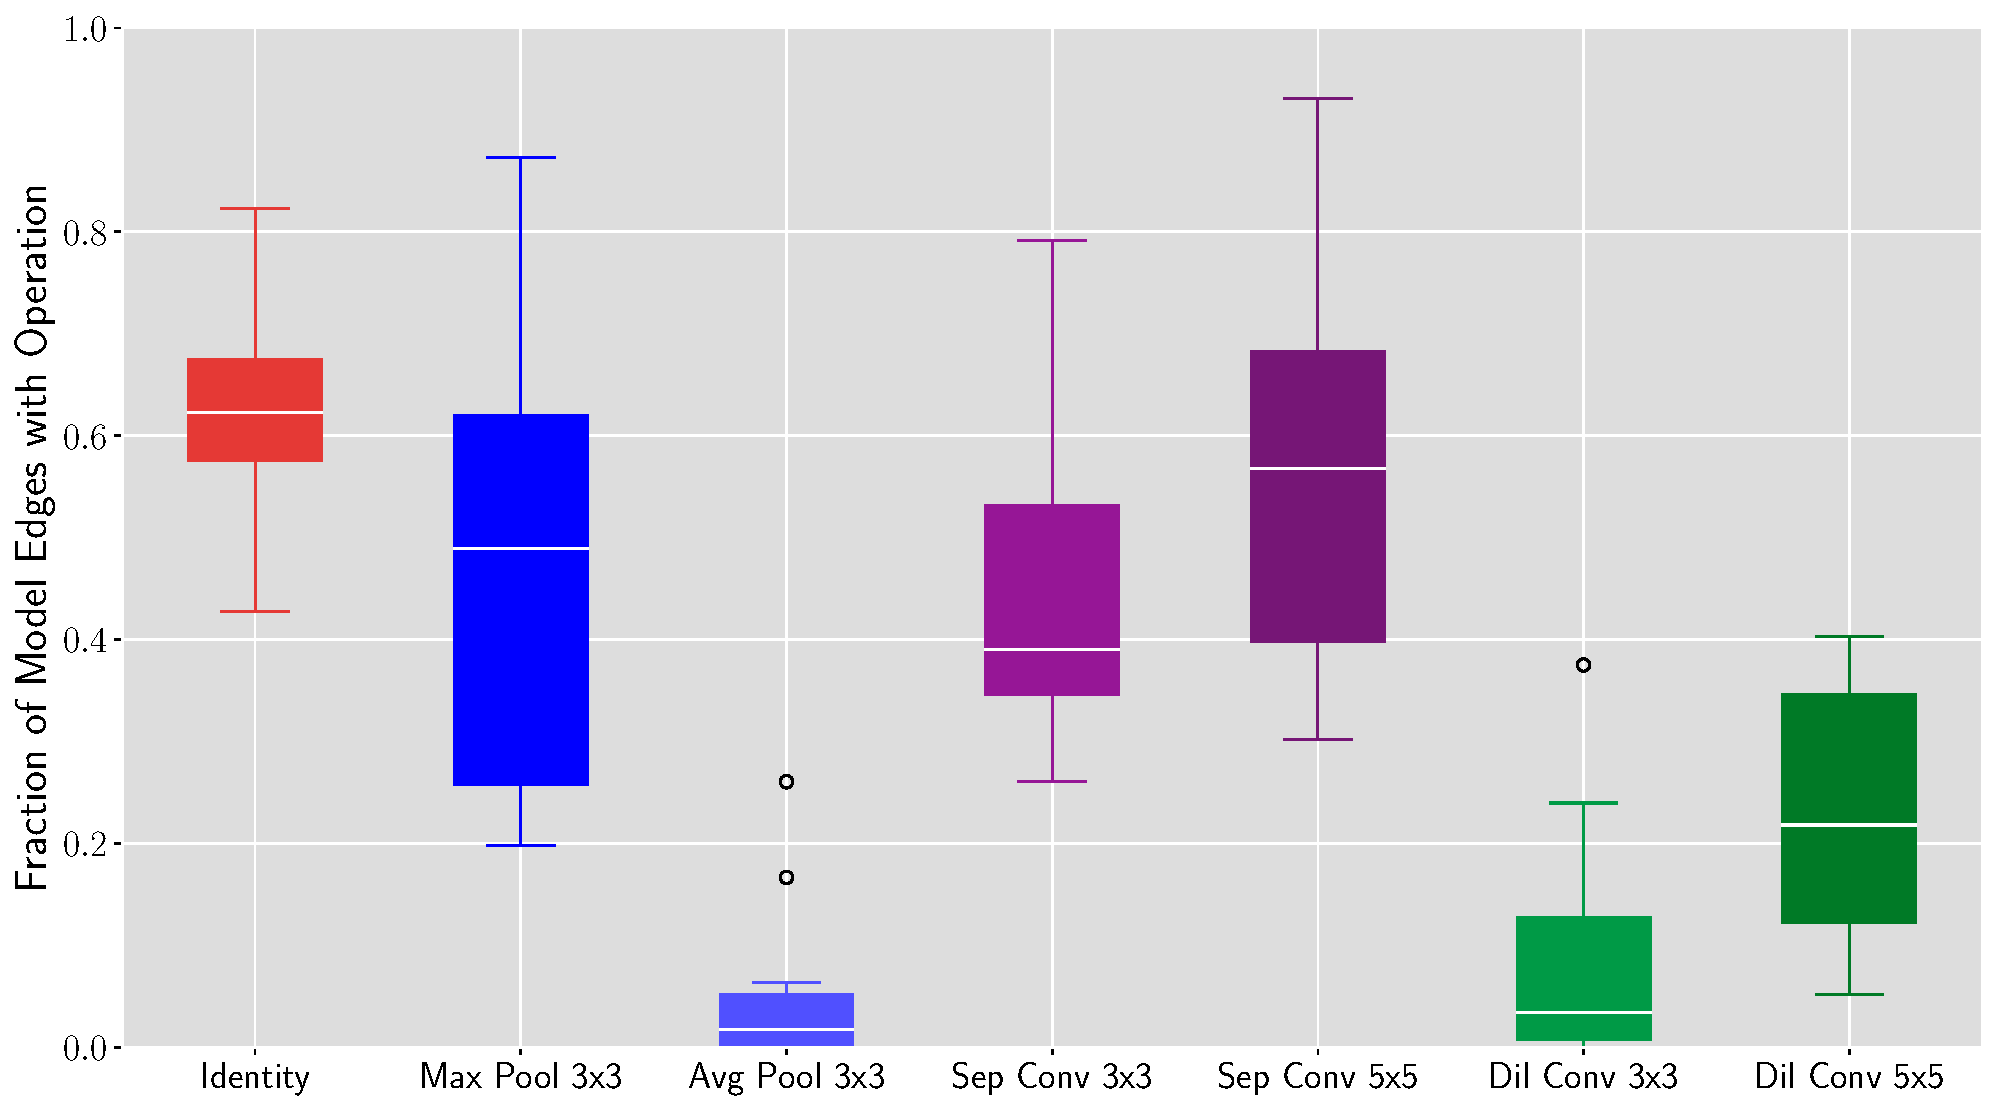
\includegraphics[width=.9\textwidth]{op_frequency}
	\caption[Fraction of edges within a single model that contain a given operation]{Fraction of edges within a single model that contain the given operation, averaged over 12 different
	CIFAR-10 Bonsai models of various configurations. This indicates clear operational preferences, with dilated
	convolutions and average poolings the least favored. }
	\label{fig:opfreq}
\end{figure}

Notably, average poolings only appear in 1.7\% of edges in the median model;
this corresponds to about once per model. 3x3 dilated convolutions are similarly
unpopular, showing up in only 3.4\% of the edges in the median model. On the other hand, identities, 3x3 max
poolings and separable convolutions are highly preferred, with one model selecting 5x5 separable convolutions in as many as
93\% of its edges. One way to explain this consistency across all 12 models is that it could be due
to simply the compression loss weightings of each operation by size, that the preferred operations are smaller in VRAM
size and thus their presence is less heavily penalized in the loss function. Conversely, it would also be expected that the
least popular operations would be the largest and most heavily penalized. However, as Table~\ref{tab:allopcosts} shows,
this is not the case; average poolings are the second smallest operation in the space, while dilated convolutions
are third smallest. Despite these operations being the second and third `easiest' to keep, they are
systematically removed from the models. On the other hand, separable convolutions are the largest operation by almost
twofold, yet the models are more than willing to pay this price. This is all indicative of some separate reasoning beyond
pure compression loss penalties.

\begin{figure}[ht]
	\centering
	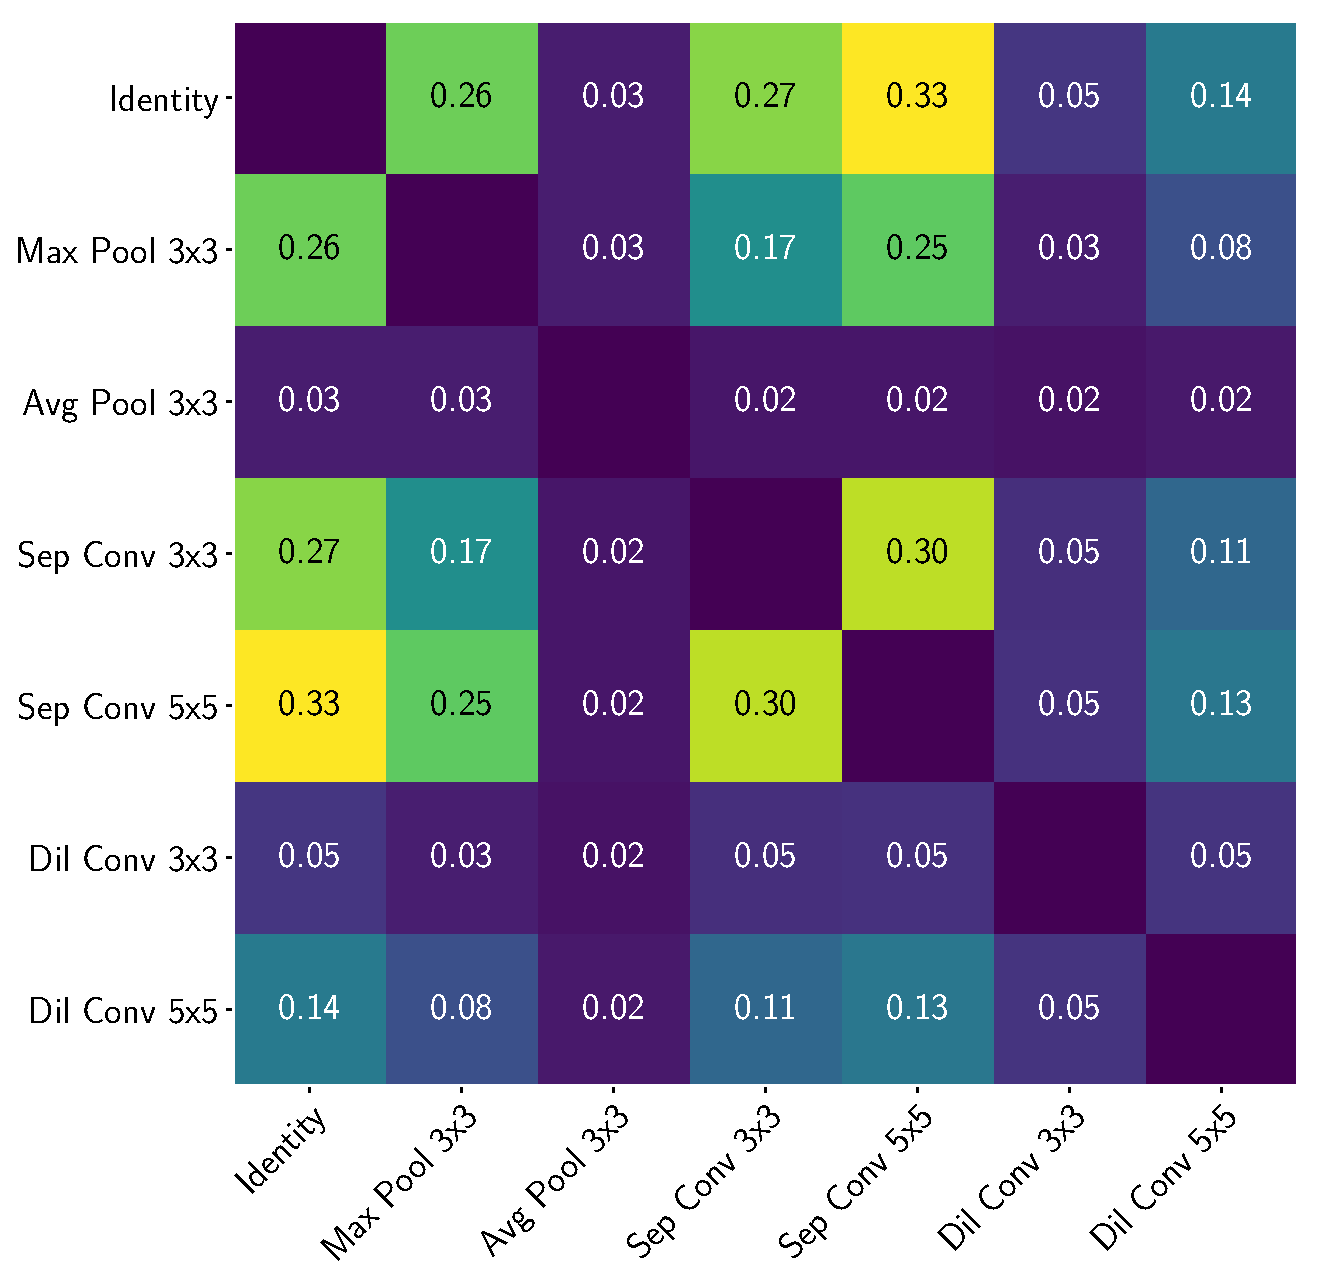
\includegraphics[width=.7\textwidth]{op_cooccurence}
	\caption[Frequency of operation co-occurrence within an edge]{Frequency of operation co-occurrence within an edge, aggregated over 12 different
	CIFAR-10 Bonsai models of various configurations.The most common pairing is
		[Identity, 5x5 Separable Convolution], which occurs in 355 of 1062 edges or 33\% of the time.}
	\label{fig:op_coocurrence}
\end{figure}

Next is operation co-occurrence; how often operations appear together in the same edge. Here,
all 1062 edges within the 12 examined models are examined, and measure the frequency by which any pair of operations
appear together within those 1062 edges. This is presented in Figure~\ref{fig:op_coocurrence}. Interestingly, the first
and third most common operation co-occurrences are [Identity-5x5 Separable Convolution] and
[Identity=3x3 Separable Convolution] respectively. Such an edge constituting of either pair of operations
exactly matches the connectivity pattern of ResNet models, that is, parallel identity and separable convolutions that
are subsequently summed together. The optimistic perspective on this outcome is that BonsaiNet organically discovered
residual connections on its own, isolating those two particular patterns as its favorites among the 49 possible
operation pairs. This would indicate that the design intuitions it learns closely aligns with those that human network designers have
discovered, which supports that BonsaiNet designs models intelligently and deliberately, as well as demonstrates the strengths
of human design patterns. This reasoning has a natural next step, which is that if some of BonsaiNet's behaviors align
with the pinnacle of human design, perhaps BonsaiNet's other design proclivities align with as-of-yet undiscovered
best practices; there is potentially a wealth of design knowledge that can be gained by studying these models.

More pessimistically, it could be theorized that the implicit parallel design of the search space heavily biases the discovery
of ResNet-esque patterns, and that Identity-Separable Convolution pairs are simply the most viable option given that bias.
However, this still implies that BonsaiNet can identify good operation pairings from poor ones, which is still a meaningful
benchmark to achieve.

\section{Comparisons and Conclusions}
\begin{table}[ht!]
\begin{center}
\begin{tabular}{c|c|c|c}
 & Test Acc. & Params (M) & Search Hours\\
\hline
NAS-Net                     & 95.53\% 	                    & 7.1   		& 37,755 \\
ENAS Micro-search	        & 96.131\%            		    & 38.0  		& 7.7     \\
ENAS Macro-search		    & 97.11\%            		    & 4.6   		& 14.4    \\
DARTS First-order     	    & 97.00 $\pm$ 0.14\% 		    & 3.3   		& 36      \\
DARTS Second-order     	    & 97.24 $\pm$ 0.09\% 		    & 3.3   		& 96 \\
NAO (w/o weight sharing)    & \textbf{98.07\%} 	            & 144.6 		& 4,800 \\
NAO (w/ weight sharing)     & 97.07\%        	            & \textbf{2.5}  & 7 \\
ProxylessNAS                & 97.92\%                       & 5.7           & N/A           \\
ENAS/DARTS/NAO Random	  	& 96.48 $\pm$ 0.18\%			& -				& -\\
PC-DARTS                    & 97.43\%   	                & 3.6           & 2.4 \\
 \hline
Bonsai SC						& 96.83\% & 3.38 	& 11.50 \\
Random 1 SC						& 95.32\% & 4.54 	& -- \\
Random 2 SC						& 95.19\% & 3.68 	& -- \\
Bonsai LC1				 		& 96.69\% & 2.64 	& 2.53 \\
Bonsai LC2						& 97.04\% & 7.39	& 2.54 \\
Bonsai LC3090					& 97.07\% & 23.36 	& \textbf{1.66} \\
Bonsai LC2 (no prune, no growth)& 97.08\% & 12.04	& 0\\
Bonsai LC2 (prune, no growth)	& 97.17\% & 6.63   	& 0\\
\end{tabular}
\end{center}
\caption[CIFAR-10 statistics for all of the NAS models covered thus far, including BonsaiNet]{CIFAR-10 statistics for all of the NAS models covered thus far.
Total runtime is not consistently reported
in literature, and thus is not shown here, but in theory should be relatively consistent between similarly sized models.}
\label{tab:bonsai_comp_performance}
\end{table}

When compared against other leading NAS algorithms (see Table~\ref{tab:bonsai_comp_performance}),
some strengths of BonsaiNet become apparent. Notably, it performs
search extremely rapidly, identifying very competitive models within three hours. An important comparison here is that of
DARTS, which uses an identical GPU specification as the non-3090 BonsaiNet runs do. For example, the best Bonsai LC2 model
outperformed the DARTS First-order model, while requiring 14 times fewer search hours. The greatest advantage of BonsaiNet
however is its robustness and flexibility, in that it provides consistent
performance over various different configurations. Depending on the particular configuration, BonsaiNet models can
be optimized for whichever target is most important to the particular use-case. If desired, BonsaiNet models can aim
for raw, top-end classification performance to maximize the potential performance within a certain VRAM requirement.
Alternatively, BonsaiNet models can be designed to be highly parameter, FLOP, and time efficient, and can find optimal
architectures within those constraints. As such, BonsaiNet has the potential to be a powerful and versatile tool for use in
a broad variety of deep learning contexts.

\section{Future Work}
The main area of remaining research for BonsaiNet is further comparisons against random search in the various large
cell configurations, as well as evaluating its robustness across more diverse cellular configurations. The former
is relatively straightforward to perform; simply perform level 1 and 2 random searches in the large cell configurations
at identical compression levels as used by BonsaiNet. The latter is again relatively straightforward, simply involving
testing many different configurations for performance. The difficulty here is picking meaningful comparisons to make
with regards to configuration performance; the small-cell configuration draws direct parallels to DARTS which offers obvious
comparisons, but appropriate comparisons in the literature for more idiosyncratic configurations will be scarcer. One possible
approach is to unify both points; arbitrarily select a configuration and train a BonsaiNet model with it, then compare that to
random search. This provides an idea of the robustness of BonsaiNet in these various configurations, by showing that it
does or does not consistently outperform random search. However, each such test of either BonsaiNet or random search
takes around three or four days, which means such an experiment is very time-consuming and thus had to be deprioritized versus
other experiments.

Another potential avenue of exploration is to try and design an automatic configurator for BonsaiNet, some wrapper that
given a dataset and task chooses an optimal configuration by which to run BonsaiNet. Development of such a tool would
be benefited by the above robustness work, as data from that experiment could inform how configurational choices influence
Bonsai's performance for better or worse.

Finally, exploring the efficacy of Bonsai's growth and pruning in an unconstrained search space is an
interesting avenue to explore. That is to say, a scenario wherein the new sections added to Bonsai were not predetermined, and instead
edges were added dynamically according to the model's specific needs. This question led to the development of SpiderNet,
an extension of BonsaiNet that grows dynamically edge by edge as new space is created via pruning.

